%%% Hlavní soubor. Zde se definují základní parametry a odkazuje se na ostatní části. %%%

%% Verze pro jednostranný tisk:
% Okraje: levý 40mm, pravý 25mm, horní a dolní 25mm
% (ale pozor, LaTeX si sám přidává 1in)
\documentclass[12pt,a4paper]{report}
\setlength\textwidth{145mm}
\setlength\textheight{247mm}
\setlength\oddsidemargin{15mm}
\setlength\evensidemargin{15mm}
\setlength\topmargin{0mm}
\setlength\headsep{0mm}
\setlength\headheight{0mm}
% \openright zařídí, aby následující text začínal na pravé straně knihy
\let\openright=\clearpage

\usepackage{catchfile}

%% Pokud tiskneme oboustranně:
% \documentclass[12pt,a4paper,twoside,openright]{report}
% \setlength\textwidth{145mm}
% \setlength\textheight{247mm}
% \setlength\oddsidemargin{14.2mm}
% \setlength\evensidemargin{0mm}
% \setlength\topmargin{0mm}
% \setlength\headsep{0mm}
% \setlength\headheight{0mm}
% \let\openright=\cleardoublepage

%% Vytváříme PDF/A-2u
\usepackage[a-2u]{pdfx}
\usepackage{listings}
\def\inline{\lstinline[basicstyle=\ttfamily,keywordstyle={}]}

%% Přepneme na českou sazbu a fonty Latin Modern
\usepackage[czech]{babel}
\usepackage{lmodern}
\usepackage[T1]{fontenc}
\usepackage{textcomp}
\usepackage{multicol}
%% Použité kódování znaků: obvykle latin2, cp1250 nebo utf8:
\usepackage[utf8]{inputenc}

%%% Další užitečné balíčky (jsou součástí běžných distribucí LaTeXu)
\usepackage{amsmath}        % rozšíření pro sazbu matematiky
\usepackage{amsfonts}       % matematické fonty
\usepackage{amsthm}         % sazba vět, definic apod.
\usepackage{bbding}         % balíček s nejrůznějšími symboly
			    % (čtverečky, hvězdičky, tužtičky, nůžtičky, ...)
\usepackage{bm}             % tučné symboly (příkaz \bm)
\usepackage{graphicx}       % vkládání obrázků
\usepackage{fancyvrb}       % vylepšené prostředí pro strojové písmo
\usepackage{indentfirst}    % zavede odsazení 1. odstavce kapitoly
\usepackage{natbib}         % zajištuje možnost odkazovat na literaturu
			    % stylem AUTOR (ROK), resp. AUTOR [ČÍSLO]
\usepackage[nottoc]{tocbibind} % zajistí přidání seznamu literatury,
                            % obrázků a tabulek do obsahu
\usepackage{icomma}         % inteligetní čárka v matematickém módu
\usepackage{dcolumn}        % lepší zarovnání sloupců v tabulkách
\usepackage{booktabs}       % lepší vodorovné linky v tabulkách
\usepackage{paralist}       % lepší enumerate a itemize
\usepackage{listings}
\usepackage{fancyhdr}
\usepackage{pdfpages}
\usepackage{dirtree}
\usepackage{subfig}
\usepackage[font=small,labelfont=bf,justification=justified,format=plain]{caption}
\usepackage{pdflscape}
% \usepackage[driver=pdftex]{geometry}
% \usepackage{mathptmx}


\hyphenation{end-point}
\hyphenation{Graph-QL}
\hyphenation{ne-ideál-ním}
\hyphenation{capture-Image}


\lstdefinelanguage{JavaScript}{
  morekeywords=[1]{break, continue, delete, else, for, function, if, in,
    new, return, this, typeof, var, void, while, with, async, await, extends},
  % Literals, primitive types, and reference types.
  morekeywords=[2]{false, null, true, boolean, number, undefined,
    Array, Boolean, Date, Math, Number, String, Object, string, Promise, Response, any},
  % Built-ins.
  morekeywords=[3]{eval, parseInt, parseFloat, escape, unescape},
  sensitive,
  morecomment=[s]{/*}{*/},
  morecomment=[l]//,
  morecomment=[s]{/**}{*/}, % JavaDoc style comments
  morestring=[b]',
  morestring=[b]"
}[keywords, comments, strings]

\lstdefinelanguage{GraphQL}{
  morekeywords=[1]{type, !},
  morekeywords=[2]{ID, String},
  morekeywords=[3]{DateTime, NonNegativeInt},
  keywordstyle=[2]\bfseries,
  keywordstyle=[3]\itshape,
  sensitive,
  morecomment=[l]\#,
  morestring=[b]',
  morestring=[b]"
}

\lstset
{ %Formatting for code in appendix
  basicstyle=\footnotesize,
  numbers=left,
  stepnumber=1,
  showstringspaces=false,
  tabsize=1,
  breaklines=true,
  breakatwhitespace=false,
}

%%% Údaje o práci

\def\NazevSkoly{Gymnázium, Praha 6, Arabská 14}
% Název oboru včetně počátečního 'Obor'.
\def\NazevOboru{Obor programování}

% Název práce v jazyce práce (přesně podle zadání)
\def\NazevPrace{Parkovací systém}

% Název práce v angličtině
\def\NazevPraceEN{Parking System}

% Jména autorů
% Abecedně podle příjmení
\def\AutorPrace{Tomáš~Černý}

% Rok odevzdání
\def\RokOdevzdani{2020}
% Měsíc odevzdání
\def\MesicOdevzdani{Březen}

% Vedoucí práce: Jméno a příjmení s~tituly

% Nepovinné poděkování (vedoucímu práce, konzultantovi, tomu, kdo
% zapůjčil software, literaturu apod.)
\def\Podekovani{%
}

% Abstrakt (doporučený rozsah cca 80-200 slov; nejedná se o zadání práce)
\def\Abstrakt{%
Cílem projektu bylo navrhnout a implementovat informační systém pro správu
komerčních parkovišť, parkovišť supermarketů, obchodních center a podobných míst.
Systém je napsán moderními technologiemi a vyžaduje málo obsluhy pomocí
automatickým rozpoznáváním SPZ díky knihovně OpenALPR a levným Android
zažízením.
Systém umožňuje vytvářet flexibilní pravidla určující cenu
parkování za jednotku času, jednotky času zadarmo a jejich interval platnosti.
Také jsou schopna filtrovat vozidla na základě rozpoznané SPZ.
Zároveň umožňuje monitorovat stav v reálném čase a číst statistiky.
To vše v přehledném uživatelském rozhraní.

Systém by po několika úpravách a přidání komunikace s
platebním terminálem a závorou měl být reálně použitelný.
}
\def\AbstraktEN{%
The goal of this project was to design and implement an information system for
administration of commercial parking lots, parking lots of supermarkets,
shopping centers and similar.
The system is written using modern technologies and requires little maintenance
by automatically recognizing license plates thanks to the OpenALPR library
and cheap Android devices.
It allows to create flexible rules that specify price per unit time,
free units of time. They can also be enabled during certain time periods and
can filter vehicles by their license plate.
The administrator can also watch both live and past statistics.
All in a well-arranged user interface.

After the addition of a payment terminal and a parking barrier and some other changes,
the system should be usable in real-life.
}

% 3 až 5 klíčových slov (doporučeno), každé uzavřeno ve složených závorkách
\def\KlicovaSlova{%
{rozpoznávání SPZ}, {počítačové vidění}, {React}, {SPA}, {Typescript}, {GraphQL}
}
\def\KlicovaSlovaEN{%
{license plate recognition}, {computer vision}, {React}, {SPA}, {Typescript}, {GraphQL}
}

%% Balíček hyperref, kterým jdou vyrábět klikací odkazy v PDF,
%% ale hlavně ho používáme k uložení metadat do PDF (včetně obsahu).
%% Většinu nastavítek přednastaví balíček pdfx.
\hypersetup{unicode}
\hypersetup{breaklinks=true}

%% Definice různých užitečných maker (viz popis uvnitř souboru)
%%% Tento soubor obsahuje definice různých užitečných maker a prostředí %%%
%%% Další makra připisujte sem, ať nepřekáží v ostatních souborech.     %%%

%%% Drobné úpravy stylu

% Tato makra přesvědčují mírně ošklivým trikem LaTeX, aby hlavičky kapitol
% sázel příčetněji a nevynechával nad nimi spoustu místa. Směle ignorujte.
\makeatletter
\def\@makechapterhead#1{
  {\parindent \z@ \raggedright \normalfont
   \Huge\bfseries \thechapter. #1
   \par\nobreak
   \vskip 20\p@
}}
\def\@makeschapterhead#1{
  {\parindent \z@ \raggedright \normalfont
   \Huge\bfseries #1
   \par\nobreak
   \vskip 20\p@
}}
\makeatother

% Toto makro definuje kapitolu, která není očíslovaná, ale je uvedena v obsahu.
\def\chapwithtoc#1{
\chapter*{#1}
\addcontentsline{toc}{chapter}{#1}
}

% Trochu volnější nastavení dělení slov, než je default.
\lefthyphenmin=2
\righthyphenmin=2

% Zapne černé "slimáky" na koncích řádků, které přetekly, abychom si
% jich lépe všimli.
% \overfullrule=1mm

%%% Makra pro definice, věty, tvrzení, příklady, ... (vyžaduje baliček amsthm)

\theoremstyle{plain}
\newtheorem{veta}{Věta}
\newtheorem{lemma}[veta]{Lemma}
\newtheorem{tvrz}[veta]{Tvrzení}

\theoremstyle{plain}
\newtheorem{definice}{Definice}

\theoremstyle{remark}
\newtheorem*{dusl}{Důsledek}
\newtheorem*{pozn}{Poznámka}
\newtheorem*{prikl}{Příklad}

%%% Prostředí pro důkazy

\newenvironment{dukaz}{
  \par\medskip\noindent
  \textit{Důkaz}.
}{
\newline
\rightline{$\square$}  % nebo \SquareCastShadowBottomRight z balíčku bbding
}

%%% Prostředí pro sazbu kódu, případně vstupu/výstupu počítačových
%%% programů. (Vyžaduje balíček fancyvrb -- fancy verbatim.)

\DefineVerbatimEnvironment{code}{Verbatim}{fontsize=\small, frame=single}

%%% Prostor reálných, resp. přirozených čísel
\newcommand{\R}{\mathbb{R}}
\newcommand{\N}{\mathbb{N}}

%%% Užitečné operátory pro statistiku a pravděpodobnost
\DeclareMathOperator{\pr}{\textsf{P}}
\DeclareMathOperator{\E}{\textsf{E}\,}
\DeclareMathOperator{\var}{\textrm{var}}
\DeclareMathOperator{\sd}{\textrm{sd}}

%%% Příkaz pro transpozici vektoru/matice
\newcommand{\T}[1]{#1^\top}

%%% Vychytávky pro matematiku
\newcommand{\goto}{\rightarrow}
\newcommand{\gotop}{\stackrel{P}{\longrightarrow}}
\newcommand{\maon}[1]{o(n^{#1})}
\newcommand{\abs}[1]{\left|{#1}\right|}
\newcommand{\dint}{\int_0^\tau\!\!\int_0^\tau}
\newcommand{\isqr}[1]{\frac{1}{\sqrt{#1}}}

%%% Vychytávky pro tabulky
\newcommand{\pulrad}[1]{\raisebox{1.5ex}[0pt]{#1}}
\newcommand{\mc}[1]{\multicolumn{1}{c}{#1}}


%% Titulní strana a různé povinné informační strany
\begin{document}

%%% Titulní strana práce a další povinné informační strany

%%% Titulní strana práce

\pagestyle{empty}
\hypersetup{pageanchor=false}

\begin{center}

{\LARGE\bfseries\NazevSkoly}

\vspace{-22mm}
\vfill

{\LARGE\NazevOboru}

\vfill

\centerline{\mbox{
\includegraphics[width=100mm]{../img/logo-ga-new.pdf}}}

\vspace{-8mm}
\vfill

{\bf\Large ROČNÍKOVÝ PROJEKT}

\vfill

{\Large \AutorPrace}

\vspace{15mm}

{\LARGE\bfseries\NazevPrace}

% \vfill
% \Katedra
% \vfill

% \begin{tabular}{rl}

% Vedoucí bakalářské práce: & \Vedouci \\
% \noalign{\vspace{2mm}}

\vfill

\MesicOdevzdani \ \RokOdevzdani

\end{center}

\newpage

%%% Následuje vevázaný list -- kopie podepsaného "Zadání bakalářské práce".
%%% Toto zadání NENÍ součástí elektronické verze práce, nescanovat.

%%% Strana s čestným prohlášením k bakalářské práci

\openright
\hypersetup{pageanchor=true}
\pagestyle{plain}
\pagenumbering{roman}
\vglue 0pt plus 1fill

\noindent Prohlašuji, že jsem jediným autorem tohoto projektu, všechny citace
jsou řádně označené a všechna použitá literatura a další zdroje jsou v práci
uvedené.  Tímto dle zákona 121/2000 Sb. (tzv. Autorský zákon) ve znění
pozdějších předpisů uděluji bezúplatně škole Gymnázium, Praha 6, Arabská14
oprávnění k výkonu práva na rozmnožování díla (§ 13) a práva na sdělování díla
veřejnosti (§ 18) na dobu časově neomezenou a bez omezení územního rozsahu.

\vspace{10mm}

\hbox{\hbox to 0.5\hsize{%
V ........ dne ............
\hss}\hbox to 0.5\hsize{%
Tomáš Černý ............
\hss}}

\vspace{20mm}

% \newpage
%
% %%% Poděkování
%
% \openright
%
% \noindent
% \Podekovani

\newpage

%%% Povinná informační strana bakalářské práce

\openright

\vbox to 0.5\vsize{
\setlength\parindent{0mm}
\setlength\parskip{5mm}

Název práce:
\NazevPrace

Autoři:
\AutorPrace

% TODO: Je Lána vedoucí?
% Vedoucí práce:
% \Vedouci, \KatedraVedouciho

Abstrakt:
\Abstrakt

% Klíčová slova:
% \KlicovaSlova

\vss}\nobreak\vbox to 0.49\vsize{
\setlength\parindent{0mm}
\setlength\parskip{5mm}

% Opakování v angličtině.

Title:
\NazevPraceEN

Authors:
\AutorPrace

Abstract:
\AbstraktEN

\vss}

\newpage

\openright
\pagestyle{plain}
\pagenumbering{arabic}
\setcounter{page}{1}


%%% Strana s automaticky generovaným obsahem bakalářské práce

\tableofcontents

%%% Jednotlivé kapitoly práce jsou pro přehlednost uloženy v samostatných souborech
\chapter{Úvod} \label{uvod}

\noindent
Tento dokument se zabývá koncepcí a implementací informačního systému pro uzavřená
parkoviště s automatickým rozpoznáváním SPZ bez použití drahého kamerového hardware.
Inspirací pro projekt bylo, že se po autorovi při výjezdu z parkoviště nechtěl
parkovací lístek, nýbrž vozidlo bylo puštěno na základě SPZ.

Projekt se nezabývá operací se závorou a platebním terminálem, neb by to zvyšovalo
obtížnost už tak obtížného projektu a vyžadovalo by to poměrně vysoké
náklady na hardware.

Projekt zároveň slouží k vyzkoušení si moderních webových technologií
a frameworků s přesahem k mobilnímu vývoji a počítačovému vidění.

\section*{Zadání} \label{zadani}

\noindent
Parkovací systém má mít následující funkcionalitu:

\begin{enumerate}
  \setlength\itemsep{0.05em}
  \item Naskenování SPZ.
  \item Vytváření dostatečně flexibilních pravidel pro většinu použití.
  \begin{enumerate}
    \setlength\itemsep{0.05em}
      \item Od času A do B za tarif X/jednotka času.
      \item Různý provoz o svátcích a víkendech.
      \item Limity na hodiny zdarma.
      \item Filtrování vozidel -- pro různá vozidla mohou platit jiná pravidla.
    \end{enumerate}
  \item Statistiky počtu aut a výdělku s grafy.
\end{enumerate}


\chapter{Architektura a technologie} \label{archtech}

\section{Architektura řešení} \label{architektura_reseni}

\begin{figure} \centering
  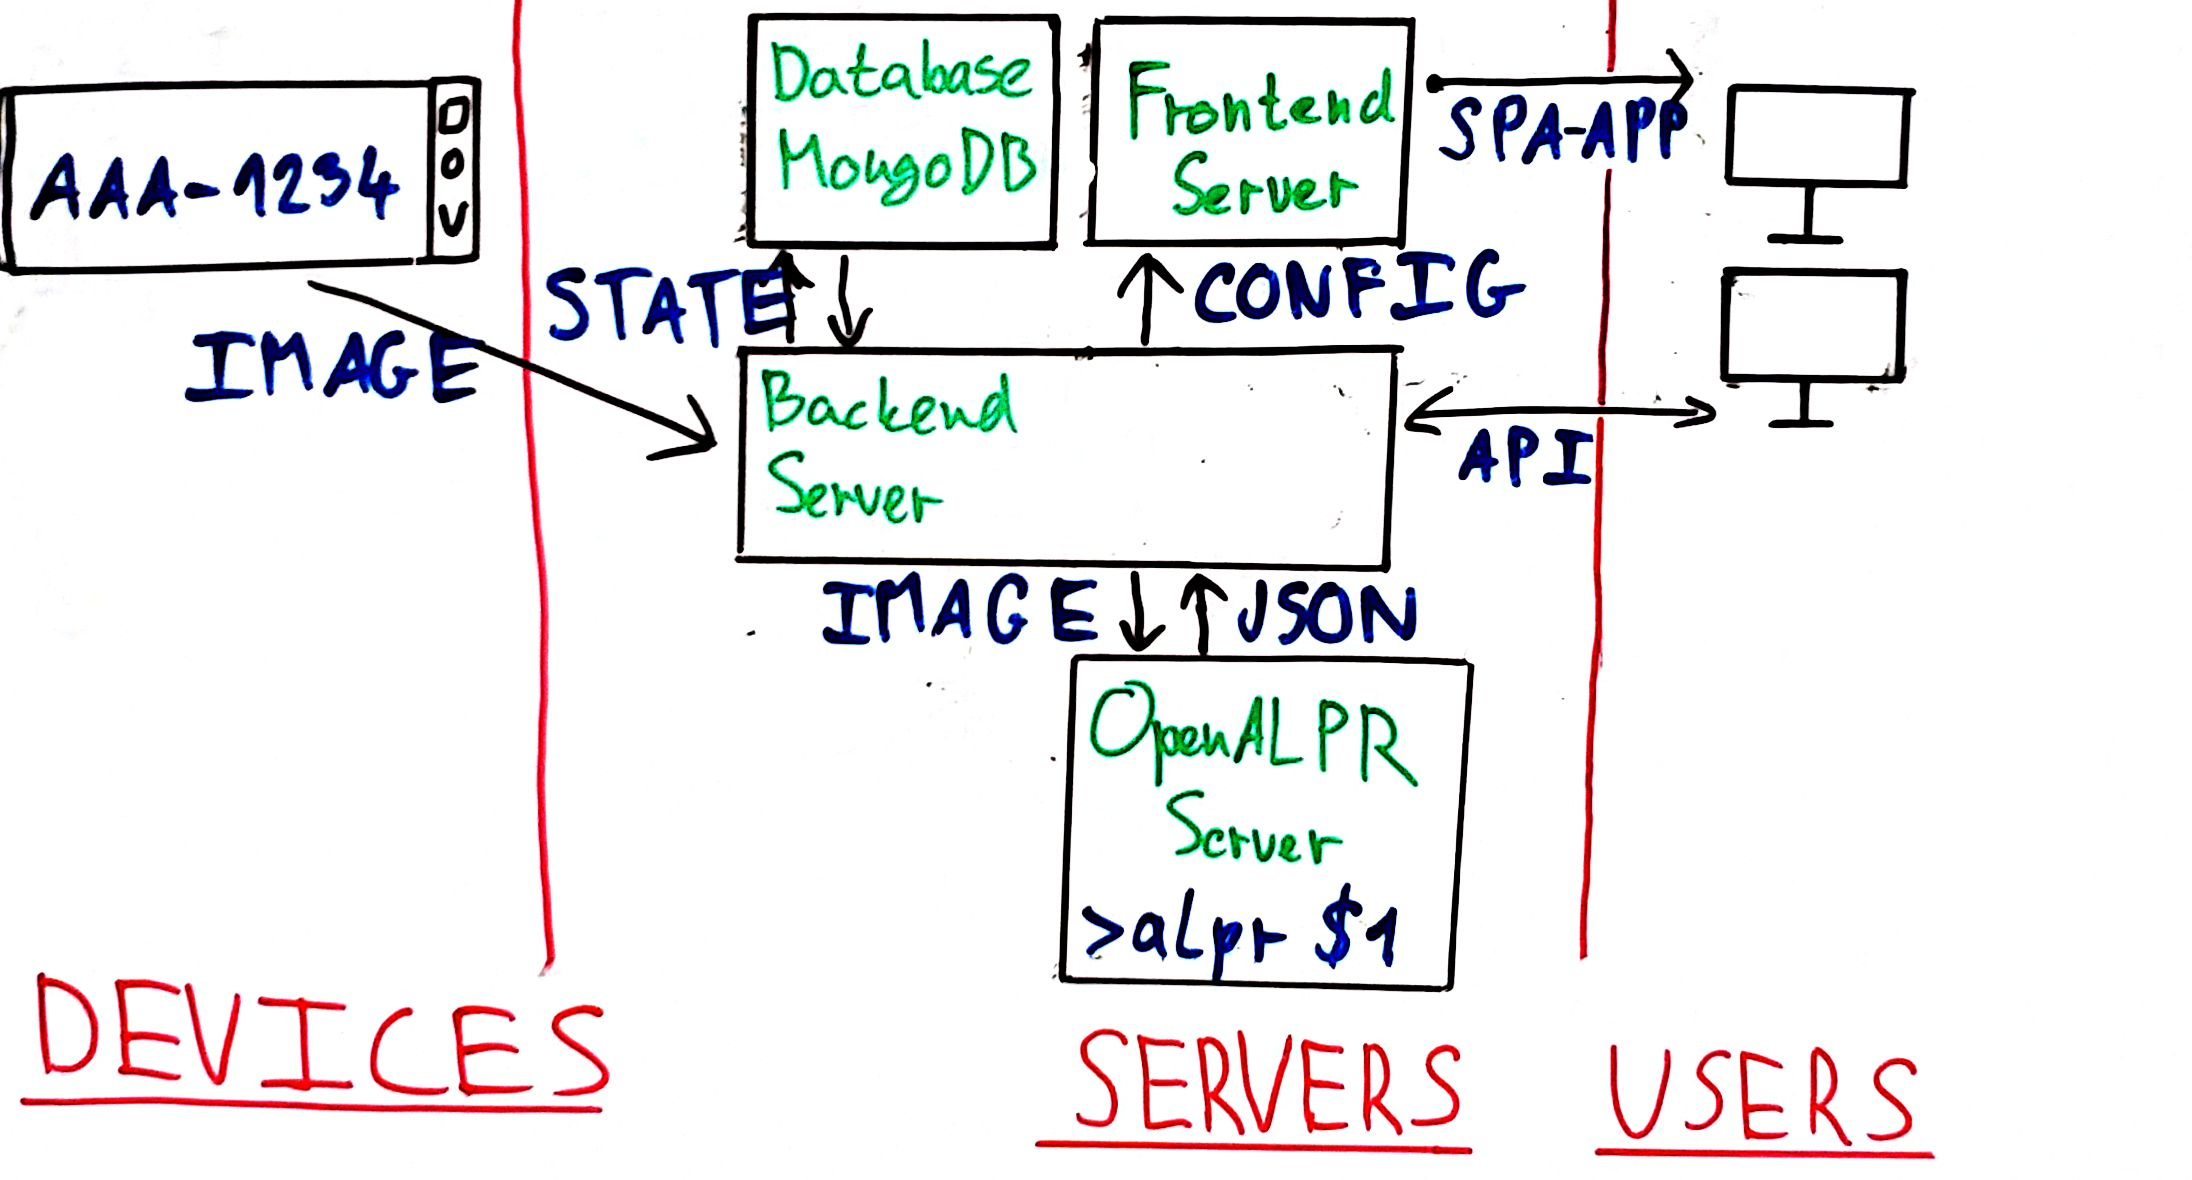
\includegraphics[width=145mm]{../img/architecture_drawing.jpg}
  \caption{Diagram komponent a jejich komunikace.}
  \label{fig:architecture_drawing}
\end{figure}

\noindent
Parkovací systém se skládá z následujících částí, které si nyní popíšeme stručně a detailněji v
následujících kapitolách.
Jednotlivé komponenty spolu komunikují pomocí HTTP.
Obrázek \ref{fig:architecture_drawing} ukazuje tyto části a nastiňuje obsah komunikace.

\begin{itemize}
  \setlength\itemsep{.05em}
  \item \textbf{Backend} je středobodem celého systému -- komunikuje se všemi ostatními komponentami.
  Zajišťuje business logiku aplikace, autentizaci i autorizaci uživatelů i zařízení
  a persistenci dat do databáze.
  \begin{itemize}
    \setlength\itemsep{.05em}
    \item \textbf{Databáze} slouží k ukládání a čtení dat.
    \item \textbf{OpenALPR Server} obstarává přístup
          ke knihovně OpenALPR přes HTTP, která rozpoznává SPZ.
  \end{itemize}
  \item \textbf{Mobilní aplikace} je určená pro platformu Android a posílá obrazová data na backend,
        kde jsou zpracována.
  \item \textbf{Frontend} je rozhraní mezi celým systémem a správcem parkoviště.
\end{itemize}

\section{Technologie}

\subsection{Databáze}

\noindent
Databáze MongoDB byla vybrána, protože data se budou převážně zapisovat a bude potřeba v nich rychle
hledat a provádět agregační dotazy.
MongoDB je takzvaná NoSQL databáze -- k dotazování se nepoužívá SQL, nýbrž vlastní způsob dotazování v
JSON. Základní datovou jednotkou je JSON/BSON dokument.
Mimo jiné umožňuje provoz několika spolupracujících instancí, zálohování apod. \citep[][]{MongoDB}

\subsection{Backend} \label{backend}

\noindent
Jako programovací jazyk pro backend byl zvolen staticky typovaný Typescript kvůli rychlosti vývoje
a množství knihoven, které poskytuje ekosystém Node.js. \citep[][]{Typescript} \citep[][]{Nodejs}

Pro definici databázových modelů a komunikaci s databází byla kvůli své vyspělosti a skvělé funkcionalitě zvolena
knihovna mongoose. \citep[][]{Mongoose}

Primárním způsobem komunikace s frontendem
je dotazovací jazyk GraphQL, který přináší ucelený popis poskytovaných dat pomocí kontroly typů a
expresivních dotazů, jejichž odpověď má stejný ``tvar'' v JSON formátu. 
Obrázek \ref{fig:graphql_example} ukazuje dotaz hledání uživatele podle jména.

\begin{figure} \centering
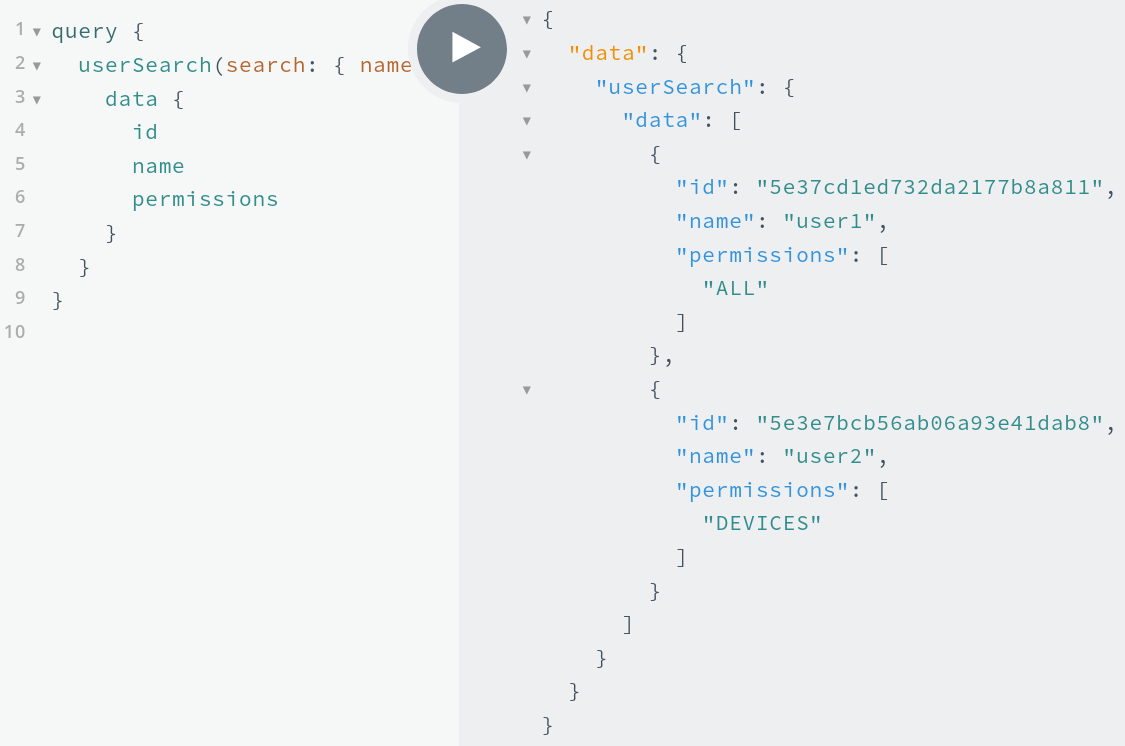
\includegraphics[width=145mm]{../img/graphql_example.png}
\caption{Příklad GraphQL dotazu (vlevo) a odpovědi (vpravo). Screenshot z nástroje GraphQL Playground.}
\label{fig:graphql_example}
\end{figure}

Model uživatele může mít i další atributy, ale GraphQL vrátí přesně ty údaje, na které se klient zeptal.
Tento triviální příklad neukazuje další funkce jako mutace dat, dědičnost typů, více dotazů v jedné HTTP žádosti
a mnoho dalších funkcí.
GraphQL je pouze specifikace vytvořená společností Facebook a má několik
implementací. \citep[][]{GraphQLDoc} Pro tento projekt byla zvolena implementace Apollo,
protože poskytuje knihovnu pro backend i frontend. \citep[][]{Apollo}

Jelikož GraphQL posílá odpovědi v JSON, není vhodné pro posílání obrázků. Je to možné za využití base64 kódování,
ale přes síť se přenese více bytů, než při použití obvyklého způsobu přes HTTP. Z toho důvodu pro posílání
obrázků bude mít backend i jiné endpointy.

\subsection{Frontend} \label{frontend}

\noindent
Pro frontend byl jako u backendu vybrán Typescript ze stejných důvodů. Webové rozhraní
je takzvaná SPA (z angl. Single-Page-Application), což znamená, že uživateli se obsah mění dynamicky
bez načítání dalších stránek.

Renderování zajišťuje knihovna React, která od klasického přístupu, kdy se odděluje HTML a Javascript do separátních
souborů, mandatuje, že v jednom souboru je jedna komponenta se vším svým HTML a logikou ve formě Javascriptu nebo
Typescriptu. \citep[][]{Reactjs}
Pomocí další knihovny typestyle pak můžeme do stejného souboru psát i typované CSS.\citep[][]{typestyle}

Aby bylo možné snadno sdílet mezi komponentami stav, byla pro takzvaný \textit{state-management} zvolena knihovna Redux.
\citep[][]{ReduxCore}
Diagram na obrázku \ref{fig:react_redux_dataflow} ukazuje tok dat mezi Reactem a Reduxem.
Tato architektura zároveň umožňuje testovatelnost -- můžeme jednoduše ověřit, zdali byla akce
například po kliknutí na tlačítko komponenty vyvolána, a jak komponenta reagovala na změnu stavu.

Jelikož je aplikace vyvíjena pro správce systému a ne pro velké množství uživatelů, můžeme si dovolit
klást menší nároky na velikost aplikace (tj. můžeme přidávat i velké knihovny), což velice usnadní vývoj.

\begin{figure}[!htb] \centering
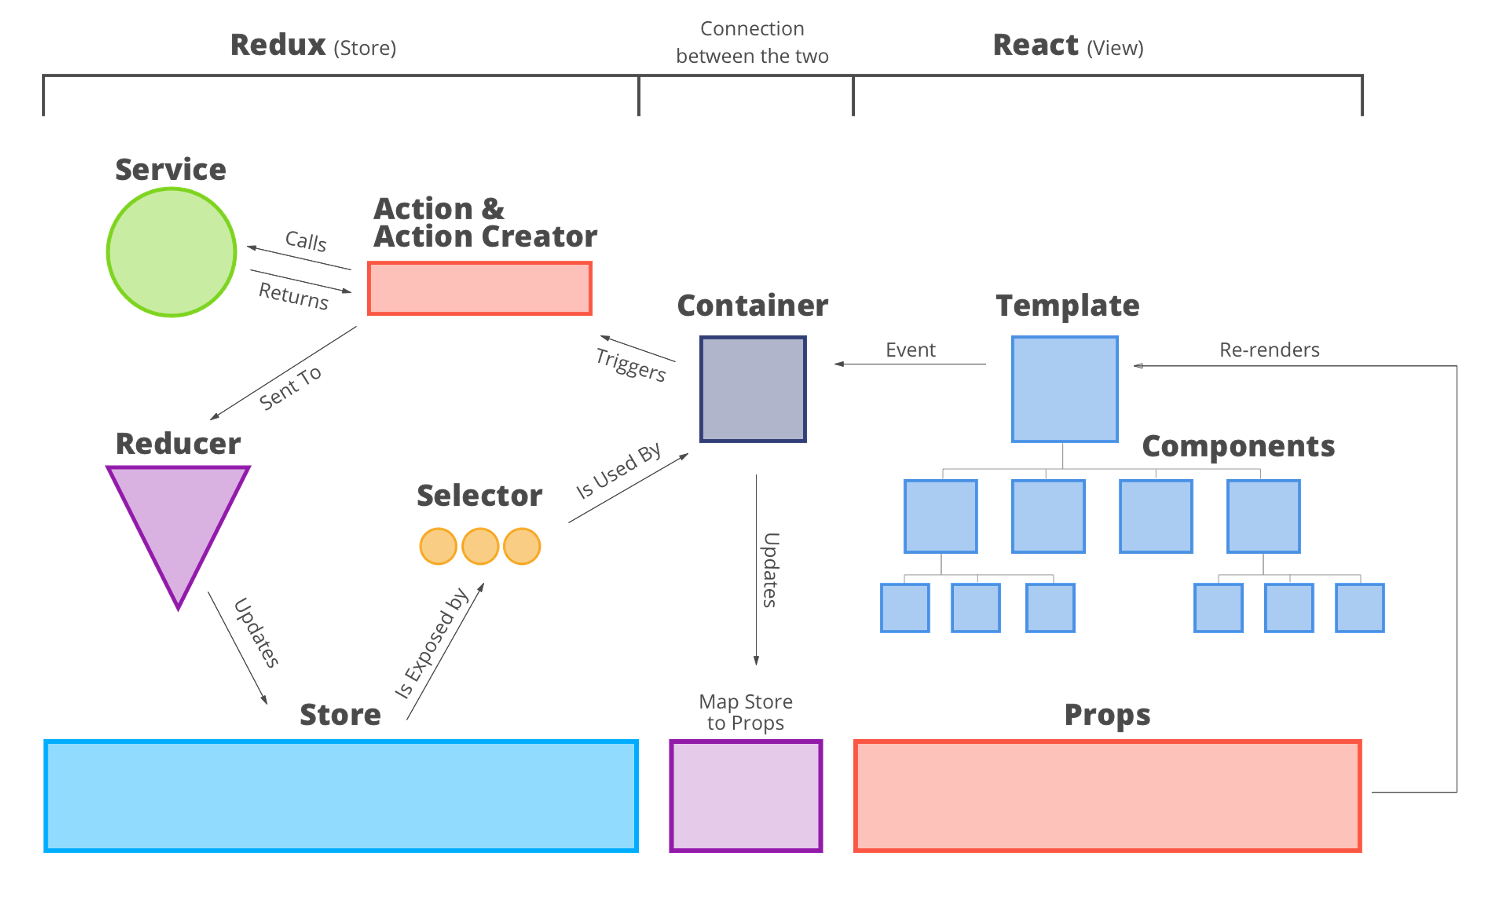
\includegraphics[width=145mm]{../img/react-redux-architecture.png}
\caption[Spojení React a Redux.]{Spojení React a Redux. \citep[][]{react_redux_dataflow}
Komponenty vyvolávají akce pomocí \textit{action-creators}, akce jsou předány prostým funkcím zvaným \textit{reducers},
ty aktualizují stav. Každá komponenta napojená
na Redux má \textit{selector} funkci, pokud se výstup z \textit{selector} funkce aktualizuje, komponenta je přerenderována Reactem.
V obrázku je prvek zvaný \textbf{Container}, ten je HOF (abbrv. Higher-Order-Function) pro komponentu a dodává jí přístup ke stavu a vytváření akcí.
Reakce na akci může být i dotaz na server nebo jiný vedlejší efekt mimo komponentu.}
\label{fig:react_redux_dataflow}
\end{figure}

\subsection{Mobilní aplikce} \label{mobile_app}

\noindent
Mobilní aplikace, která je určena pro platformu Android, měla volbu jazyka omezenou na Javu, Kotlin a C++.
Rychlost C++ není potřeba a navíc autor s tímto nízkoúrovňovým jazykem nemá takové zkušenosti.
Kotlin oproti Javě umožňuje přímočarejší přístup k prvkům uživatelského rozhraní, a proto byl zvolen.

Jediným úkolem mobilní aplikace je v pravidelném intervalu pořizovat snímky fotoaparátem a posílat je na
backend, který je patřičně zpracuje.

\subsection{Detekce SPZ}

\noindent
Detekci SPZ bude zajišťovat knihovna OpenALPR, jejímž vstupem je obrázek a popřípadě
parametry jako úhel kamery apod.
\citep[][]{OpenALPR}

Ke zbytku aplikace bude připojena malým HTTP serverem, jenž byl převzat a upraven.
Ten umožňuje poslat pomocí HTTP obrázek a obdržet JSON s SPZ daty a souřadnicemi detekované SPZ.
Samotný server ke knihovně přistupuje zavoláním binárky \textit{alpr}, který jako argument přijme cestu k
obrázku, ve kterém hledáme SPZ. \citep[][]{OpenALPR_Server}

Alternativní a lepší způsob přístupu by bylo mít v Node.js přímo takzv.
\textit{language-binding}, ale to se autorovi (a mnoho dalším, kteří se o to pokoušeli) nepodařilo.

\section{Metodika vývoje}

\noindent
Nejprve se vyvine veškerá funkcionalita v základní podobě
(na způsob MVP -- z angl. Minimal-Viable-Product) a později se vše vyhladí a zlepší. To však neznamená,
že bychom si neměli záležet na kvalitním a udržitelném kódu, naopak. Cílem je mít flexibilní základ,
na kterém lze stavět. Pro jistotu budeme psát dle uvážení automatizované testy, aby se předešlo
nežádoucímu chování aplikace po úpravě kódu -- regresi.

Backend i frontend budou vyvinuty současně. Dokud není mobilní aplikace pro zařízení, lze ji simulovat
například nástrojem \textit{curl}. Pro rychlejší prototypování bude použita technika zvaná
\textit{hot-reload}.


\chapter{Webová aplikace}

Tato kapitola popisuje zvolené postupy při psaní webové aplikace (Backend a Frontend).

\section{Obrazovky}

Dle požadavků z úvodu mějme po příhlášení do webového rozhraní následující obrazovky, mezi kterými bude uživatel přepínat pomocí hlavního menu.

\begin{itemize}
  \item \textbf{Dashboard} -- jednoduché shrnutí nedávných statistik, kolik vozidel je
        momentálně na parkovišti, aktivní zařízení apod.
  \item \textbf{Statistiky} -- detailněji zobrazené údaje o počtu parkování a výdělku podle roku, měsíce a dne s grafy.
        Zde půjde i exportovat data to CSV souboru (\textit{Comma-Separated-Values}).
  \item \textbf{Pravidla a Filtry} -- definice parkovacích pravidel a filtrů vozidel (popsáno v \ref{analysis_parking_schema}).
        Pro ověření půjde si parkovací pravidla a filtry odsimulovat.
  \item \textbf{Zařízení} -- správa zařízení zachycujících fotografie SPZ, která lze autentifikovat do systému pomocí
        QR kódu.
  \item \textbf{Správa uživatelů} -- přidávání, odebírání a úprava uživatelů a jejich operávnění.
  \item \textbf{Správa účtu} -- změna údajů a hesla současně přihlášeného uživatele.
\end{itemize}

Na obrázku \ref{fig:structure_backend} a obrázku \ref{fig:structure_frontend} je
vidět adresářová struktura Backendu a Frontendu.

\begin{figure}
  \begin{minipage}{0.45\textwidth}
    \dirtree{%
    .1 frontend.
    .2 config.
    .3 types.
    .3 utils.
    .3 webpack.
    .2 src.
    .3 app.
    .4 apis.
    .4 components.
    .4 constants.
    .4 containers.
    .4 helpers.
    .4 images.
    .4 layouts.
    .4 models.
    .4 pages.
    .4 redux.
    .4 routes.
    .4 sagas.
    .4 selectors.
    .2 translations.
    }
    \caption{Adresářová struktura Frontend.}
    \label{fig:structure_frontend}
  \end{minipage}%
  \hfill
  \begin{minipage}{0.45\textwidth}
    \dirtree{%
    .1 backend.
    .2 config.
    .2 scripts.
    .2 src.
    .3 apis.
    .3 auth.
    .3 cache.
    .3 db.
    .3 endpoints.
    .3 scripts.
    .3 types.
    .3 utils.
    .2 test\_assets.
    .2 typings.
    }
    % Disgusting but it works -- aligned
    \hfill
    \\
    \\
    \\
    \\
    \\
    \\
    \caption{Adresářová struktura Backend.}
    \label{fig:structure_backend}
  \end{minipage}%
\end{figure}

\section{GraphQL resolvery}

Protože GraphQL je primárním způsobem komunikace mezi Frontend a Backend, stojí za to si vysvětlit základní stavební bloky
GraphQL -- resolvery, které tvoří strom. Vzpoměňme si na příklad z přechozí kapitoly na obrázku \ref{fig:graphql_example}.
Zde kořenem stromu je resolver \textit{userSearch}, jenž přijímá argumenty potřebné pro jeho běh, ty jsou v tomto případě
povinné (ale nemusí). Kořenový resolver vrací nějaký typ, v tomto případě typ \textit{UserSearchResult}, který udává nalezené
uživatele (\textit{UserSearchResult.data}) a stránkování (v příkladu vynecháno).
Při návrhu tohoto resolveru bychom si mohli rozmyslet, že údaje o stránkování vynecháme a vrátíme pouze
pole nepřázdných uživatelů -- typ \textit{[User!]}.
Typ \textit{User} má v sobě také nějaké hodnoty a vrátí se nám jen ty, na které se zeptáme. Měl-li by typ \textit{User}
další objekty, mohli bychom se zeptat i na jejich hodnoty. Kdybychom psali aplikaci pro veterinární kliniku, mohli bychom se zeptat
třeba na jména mazlíčků.
Jak toto implementujeme? Pro každý kořenový resolver musíme napsat funkci, která buď přímo vrátí požadovaný objekt a nebo
k typu, který náš kořenový resolver vrací, napíšeme další resolvery. Čili kdybychom se databáze ptali na uživatele i s
mazlíčky (v SQL terminologii bychom provedli JOIN), tak bychom nemuseli pro typ \textit{User} psát resolver pro mazlíčky.
Ale kdybychom se za účelem zrychlení aplikace ptali pouze na uživatele, tak bychom museli mít jěště resolver pro mazlíčky, abychom
podporovali dotazy na mazlíčky uživatelů, což by způsobilo více poslaných dotazů do databáze, ale pokud by výkon byl problém,
můžeme se podívat přímo na jaké hodnoty se uživatel ptá.
\citep[viz][]{GraphQLDoc}

Jelikož se většina operací nad modeli se opakuje, byli napsány obecné resolvery jako HOF (Higher-Order-Function)
pro vytváření, úpravu, mazání, vyhledávání a získávání modelů v relaci.
Měnící se část je pak pouze definice databázového modelu. Díky GraphQL nemusíme ani ověřovat datové typy, které dostaneme od klienta --
GraphQL toto udělá za nás díky schema, které tvoříme my.

\section{Autentizace a autorizace} \label{auther_authen}

Autentifikace lidských uživatelů probíhá pomocí standardního hesla a zařízení pomocí dlouhého, náhodně generovaného hesla,
které je posíláno na Frontend ve formě QR kódu, které zařízení naskenuje.
Po úspěšné autentizaci obdží klient token, který kdyby klient posílal v souboru Cookie,
tak bychom se vystavovali riziku útoku CSRF/XSRF.
Místo toho bude klient posílat token v hlavičce \textit{Authorization}.

Podle tokenu klienta jednoznačně identifikujeme a víme jeho oprávnění. Endpointy a GraphQL resolvery zabezpečíme tak,
že každý endpoint nebo resolver, který vyžaduje oprávnění, dáme jako argument HOF (Higher-Order-Function)
\textit{checkPermissions} společně s požadovanými oprávněními. \textit{checkPermissions} pak zavolá původní endpoint
nebo resolver pouze pokud má klient dostatečná oprávnění.

\section{Business logika}

\subsection{Parkovací pravidla} \label{analysis_parking_schema}

\begin{itemize}
  \item Různá vozidla mohou podléhat ruzným pravidlům.
  \item Pravidla mají prioritu.
  \item Pravidla mají časové omezení.
  \item V jednu chvíli může platit více pravidel.
\end{itemize}

Mechanismus, kterým umožníme vozidlům být ovlivněna některými pravidly,
budou filtry.
Pro dostatečnou flexibilitu je zapotřebí oddělit samotná pravidla od jejich
priority, časového intervalu platnosti i filtrů,
k čemuž bude sloužit objekt typu \texttt{ParkingRuleAssignment}.

% TODO - add a db schema image that takes less space
\begin{lstlisting}
type ParkingRuleAssignment {
  rules: [ParkingRule]!
  start: DateTime!
  end: DateTime!
  # ALL nebo NONE
  vehicleFilterMode: VehicleFilterMode!
  vehicleFilters: [VehicleFilter!]
  priority: NonNegativeInt!
}

type VehicleFilter {
  id: ID!
  name: String!
  action: VehicleFilterAction!
  vehicles: [Vehicle!]!
}
\end{lstlisting}

Filtrování bude mít dva módy: začneme se všemi vozidly (ALL) a začneme bez vozidel (NONE).
Následné filtry mohou buď přidávat, nebo odstraňovat jednotlivá vozidla.
Hodí se mít filtry uložené separátně, aby mohli být využity několikrát.

Pro zjednodušení algoritmů, uvalíme omezení: ve stejný čas nesmí existovat více \texttt{ParkingRuleAssignment}
se stejnou prioritou.

\subsubsection*{Algoritmus filtru vozidel}

\textit{Vstup: objekt \texttt{ParkingRuleAssignment}, vozidlo}

\textit{Výstup: boolean určující platnost}
\begin{enumerate}
  \item Na základě módu filtrování si budeme udržovat množinu buď odstraněných vozidel (mód ALL), nebo přidaných vozidel (mód NONE).
  \item Podle příslušné akce filtrů (odstranit nebo přidat) budeme množinu našich vozidel manipulovat. Např. je-li mód ALL a filtr odstraňuje, do množiny si vozidla přidáme.
  \item Pokud je vozidlo ve výsledné množině, tak pro něj \texttt{ParkingRuleAssignment} platí pokud je filtrovací mód NONE a neplatí pokud je mód ALL. Opačné výsledky nastanou, pokud vozidlo v množině není.
\end{enumerate}

Časová i paměťová složitost algoritmu je ${\cal O}(N)$, kde $N$ je počet filtrů.

Tento algoritmus lze potenciálně rozdělit na předvýpočet (kroky 1. a 2.) a ověření (krok 3.).
To je jedna možnost, která zvýší paměťovou náročnost, protože bychom si museli pamatovat množiny, což je nepraktické.
Je-li uživatel příčetný, počet použitých filtrů nebude obrovský, a tudíž je lepší zvolit následující způsob cachovaní.
Zapamatujeme si výsledky pro určitý seznam filtrů pro konkrétní vozidlo pouze při běhu algoritmu, který je
vysvětlen v následující kapitole, čímž následující algoritmus zrychlíme.

\subsubsection*{Algoritmus pro aplikaci ParkingRuleAssignmentů}

\begin{figure}[!htb] \centering
  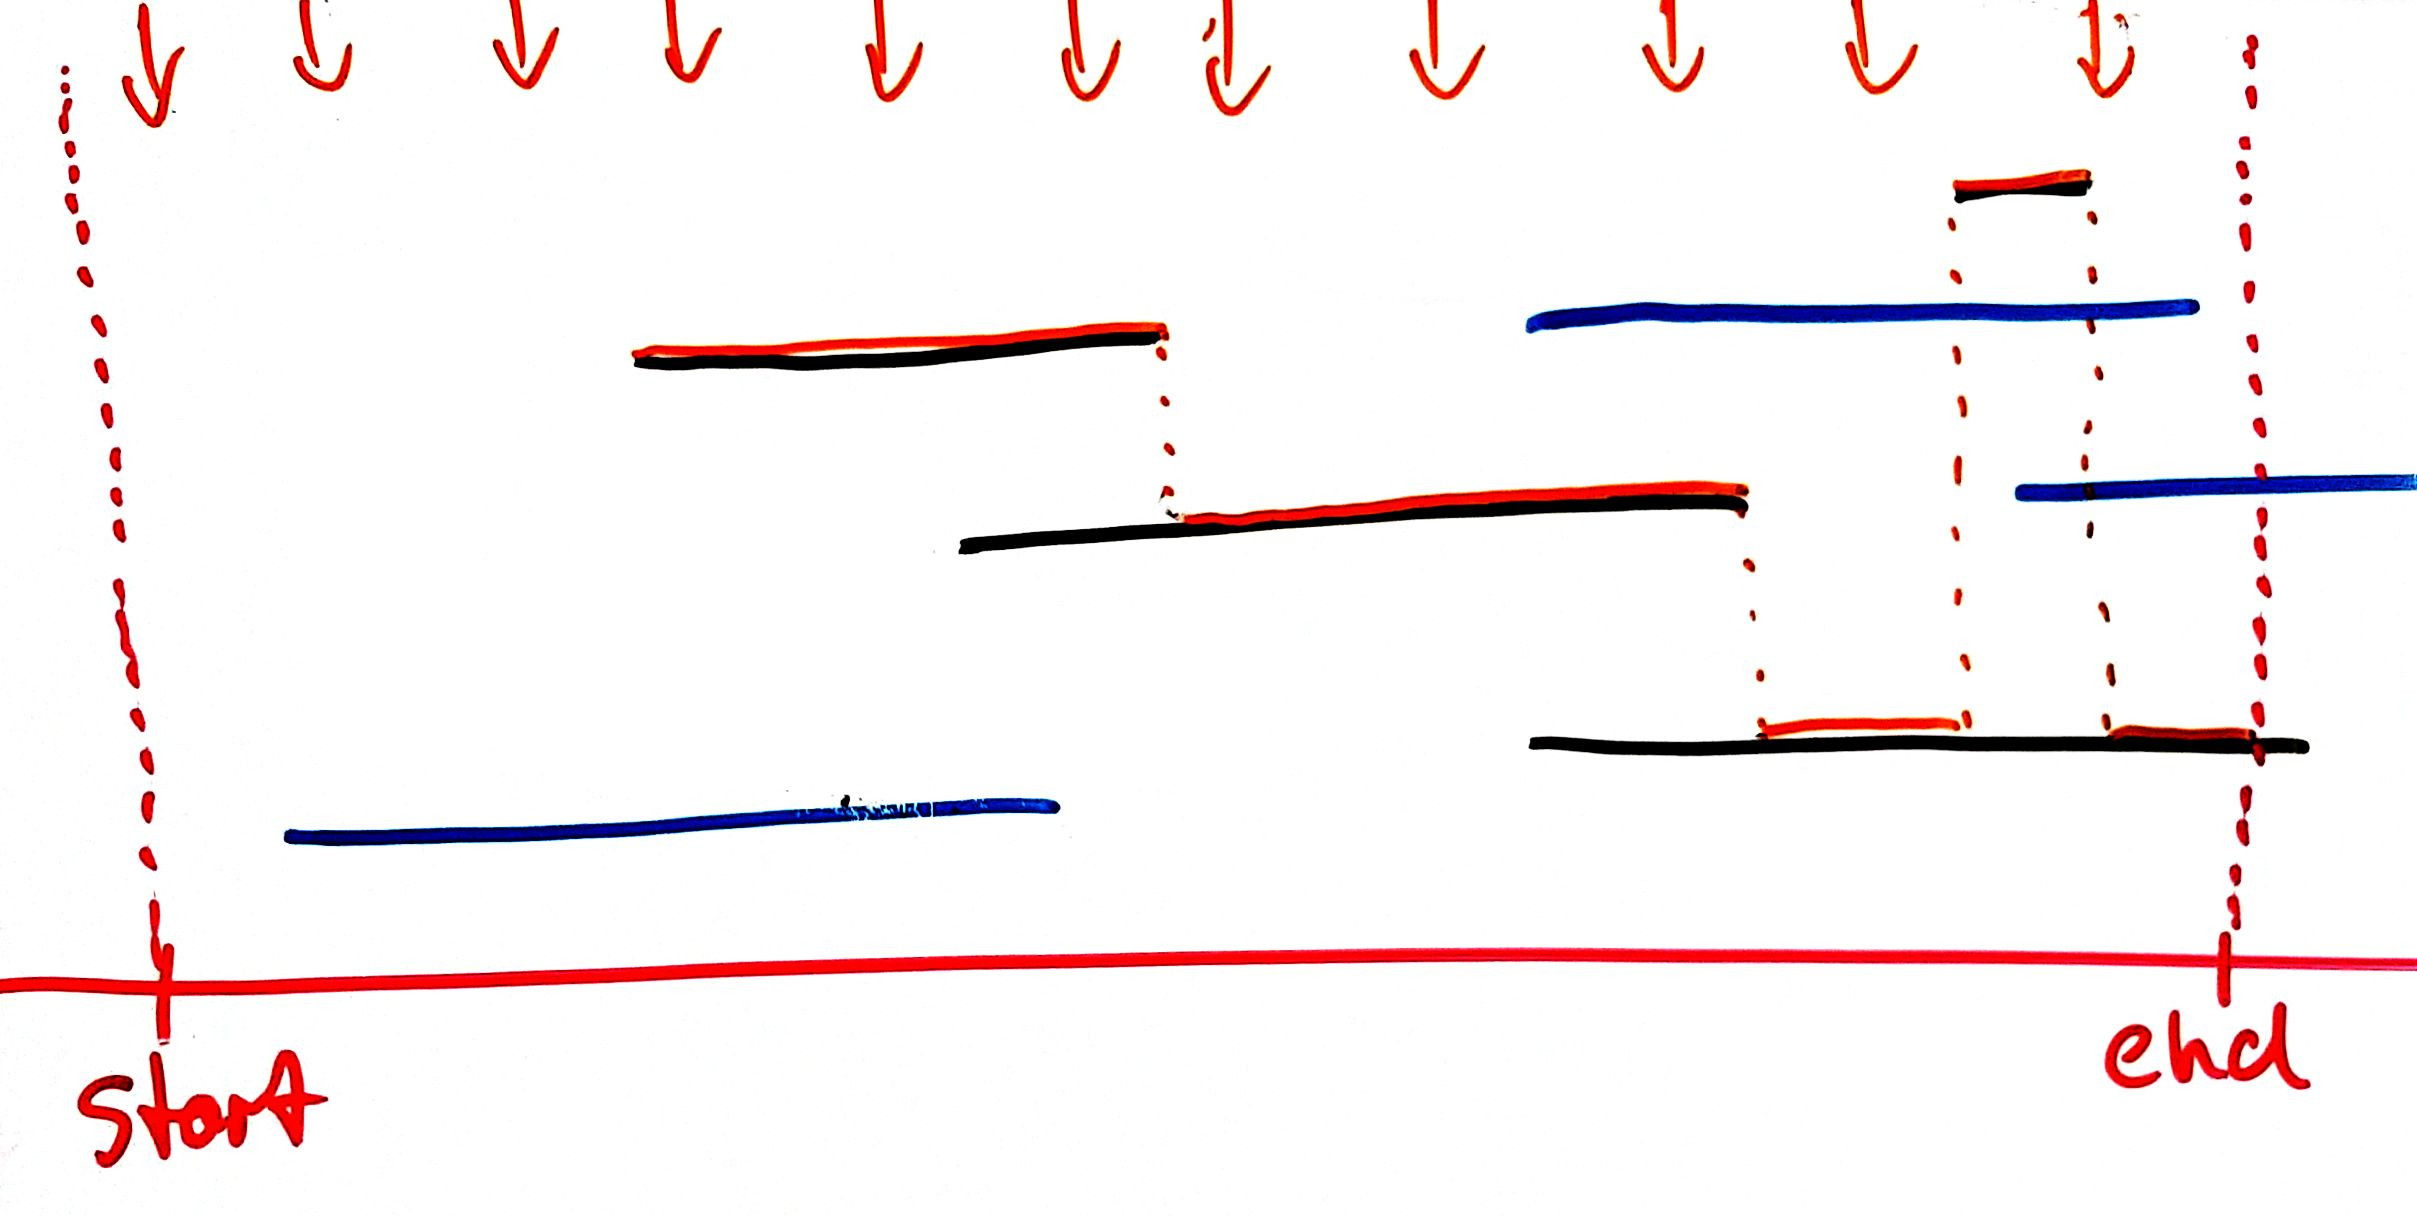
\includegraphics[width=145mm]{../img/rules_drawing.jpg}
  \textit{Modré úsečky neplatí kvůli filtrům nebo protože jsou deaktivované. Oranžová čára značí výstup požadovaného algoritmu.}
  \caption{Ilustrace problému úseček.}
  \label{fig:rules_drawing}
\end{figure}

V jednom čase může existovat více objektů typu \texttt{ParkingRuleAssignment} avšak s různou prioritou.
Může se stát, že aplikovaných \texttt{ParkingRuleAssignment} bude několik (různé priority, vyprší platnost, etc.).

Situaci si lze představit jako několik úseček navzájem rovnoběžných úseček v různých výškách, které se neprotínají.
Nás nyní zajímá, na které a v jakých intervalech na ně dopadne světlo, pokud na ně kolmo zeshora posvítíme.
Situaci lze vidět na obrázku \ref{fig:rules_drawing}.

Pro zjednodušení předpokládejme, že všechny \texttt{ParkingRuleAssignment}, které zpracováváme, platí pro naše vozidlo.
Přidat tuto kontrolu později je triviální.

\textit{Vstup: seznam \texttt{ParkingRuleAssignmentů} odpovídající pro interval pobytu vozidla na parkovišti, vozidlo}

\textit{Výstup: seznam \texttt{ParkingRuleAssignmentů} s časy platnosti}
\begin{enumerate}
  \item Seřadíme si začátky a konce úseček podle jejich času.
  \item Vytvoříme si haldu pro odkládání úseček, která řadí podle priority -- větší výše.
  \item Vytvoříme si seznam aplikovaných pravidel s časy (časy mohou se lišit od počátečních i koncových časů).
  \item Nechť \textit{s} je současná úsečka a \textit{$t_s$} čas zvolení \textit{s} (čas zvolení se může lišit od začátku úsečky).
  \item Pro každou událost \textit{u} značící začátek/konec úsečky (aplikaci pravidla) \textit{p}:
  \begin{enumerate}
    \item Pokud se jedná o začátek nové úsečky:
    \begin{enumerate}
      \item Pokud není zvolená úsečka:\\
            \textit{$t_s$} $\leftarrow$ \textit{p.start}\\
            \textit{s} $\leftarrow$ \textit{p}
      \item Pokud je zvolená úsečka a \textit{p} má vyšší prioritu než \textit{s}:\\
            \textit{s} dáme do seznamu aplikovaných pravidel se začátkem \textit{$t_s$} a koncem \textit{p.start}.\\
            \textit{s} dáme na haldu, pokud \textit{s.end} > \textit{p.end}.\\
            \textit{$t_s$} $\leftarrow$ \textit{p.start}\\
            \textit{s} $\leftarrow$ \textit{p}
      \item Pokud je zvolená úsečka a \textit{p} má nižší prioritu než \textit{s} a \textit{p.end} > \textit{s.end}:\\
            \textit{s} dáme na haldu
    \end{enumerate}
    \item Jinak (jedná se o konec nějaké úsečky):
    \begin{enumerate}
      \item Přidáme \textit{s} do seznamu aplikovaných pravidel se začátkem \textit{$t_s$} a koncem \textit{s.end}.
      \item Taháme z haldy, dokud nedostaneme úsečku s koncem později než konecm \textit{p}, nebo dokud halda není prázdná.
      \item Pokud jsme z haldy vhodnou úsečku vytáhli, použijeme ji. V opačném případě vyprázdníme \textit{s} a \textit{$t_s$}.
    \end{enumerate}
  \end{enumerate}
\end{enumerate}

Algoritmus zajisté doběhne, protože máme konečný počet událostí a v každém cyklu jednu zpracujeme.
Paměťová složitost je zřejmě lineární. Časová složitost bez filtrování je ${\cal O}(N\cdot{logN})$, kde $N$ je 
počet úseček, protože
využijeme některého z rychlích zaření a protože použijeme binární haldu a lepší. Počet operací nad haldou,
který by konečnou složitost mohl změnit, je naštestí lineární. Největší počet operací nad haldou dostaneme tak, že
každou přidanou úsečku umístíme tak, aby při zpracování jejího konce i začátku došlo k přidání a odebrání z haldy
(nejedná o tu samou úsečku). Jedna z takovýchto uspořádání je například pyramida, popřípadě zikkurat.
Tedy s každou přidanou úsečkou se počet operací nad haldou zvýší maximálně o $2$.

Přidáme-li filtrování, tak v nejhorším případě budeme ověřovat platnost každé úsečky. Bude-li $M$ průměrný počet
filtrů, pak je časová složitost ${\cal O}(N\cdot{M})$. 
% Při rozumném počtu \texttt{ParkingRuleAssignment} v daném intervalu je algoritmus velice rychlý

\section{Databázový model}

\section{Uživatelské rozhraní}

Jelikož autor neměl zkušenosti s vývojem webového uživatelského rozhraní, rozhodl se využít starter projekt
společnosti Crazy Factory, který pojí vybrané technologie dohromady a mandatuje projektu strukturu.
Navíc podporuje překlady, reportování chyb apod., což vytvářet z ničeho je obtížné. \citep[viz][]{CFProj}

\subsection{Redux a persistence stavu}

Jak již bylo zmíněno v předchozí kapitole, uživatelské rozhraní používá Redux pro sdílení stavu mezi komponentami.
Stav v Redux je strom, jenž je upravován akcema. Akce jsou předány takzvaným \textit{reducers}, což jsou prosté funkce,
jejichž vstupem je současný stav a akce a jejichž výstupem je stav nový. \citep[viz][]{ReduxCore}
Prostost reducerů umožňuje testovatelnost.

Jako příklad konkrétního využití budiž uložení některých údajů obrazovek mezi přepnutí obrazovek,
sdílení vozidla mezi stránkou s vozidly a stránkou s pravidly, schopnost seznamu parkování zvolit vozidlo a mnoho dalších.

K tomu abychom mohli uložit stav aplikace po zavření okna, použijeme knihovnu \textit{redux-persist}, která poskytuje
HOF funkci, které dáme resolver, a ona změny, které způsobí, někam uloží. V našem případě se jedná o \textit{localstorage}.

\subsection{Obecná vybírátka modelů}

Dle principu neopakování se bylo vytvořeno několik obecných UI komponent, které umožňují vyhledávání libovolných
modelů a jejich volbu a využití v ostatních komponentách. Ve zdrojovém kódu je implementujeme jako
HOF (Higher-Order-Function), což je funkce vracející další funkce -- konkrétní komponenty.
Měnící se části, které do těchto obecných komponent budeme vkládat je komponenta renderující jediný model
(\textit{renderModel}),
GraphQL dotaz pro získávání modelů (\textit{queryString}), funkce, jejímž vstupem je odpověď na GraphQL dotaz a výstupem je
samotné pole modelů (\textit{modelArrayGetter}), a funkce, jejímž vstupem je dotazovací řetězec a výstupem jsou
argumenty pro GraphQL dotaz (\textit{identifierToOptions}).

Obrázek \ref{fig:picker_lifecycle} ukazuje tok dat v jednom z obecných vybírátek.
Obrázek \ref{fig:picker_component} ukazuje vyrenderovanou komponentu téhož vybírátka.

Další vybírátka abstrahují i vstup od uživatele, takže lze použít například kalendář.

\begin{figure}[!htb] \centering
  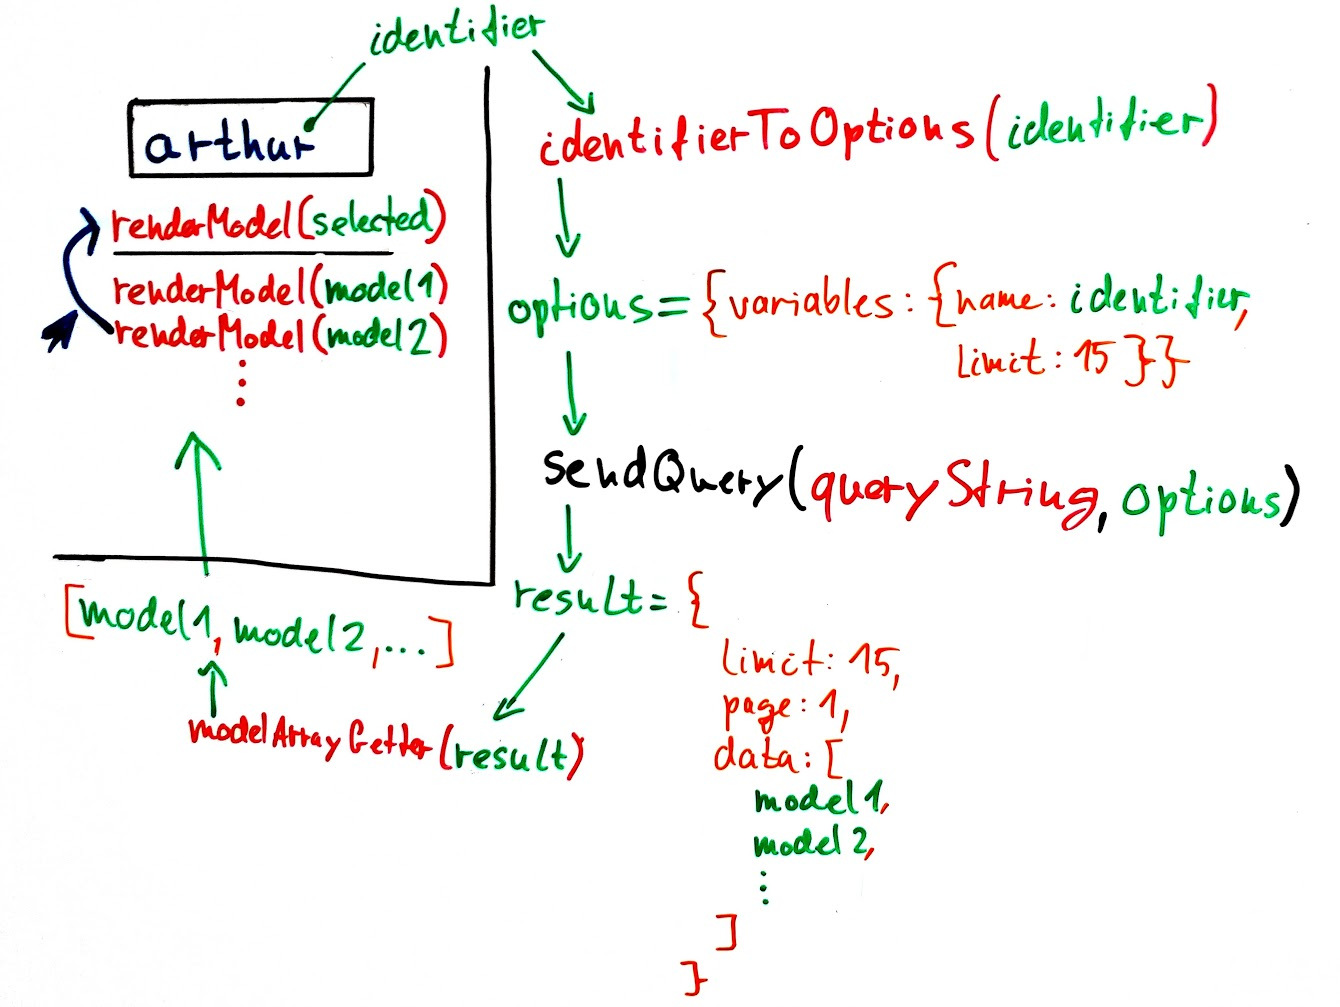
\includegraphics[width=145mm]{../img/picker_lifecycle.jpg}
  \caption{Tok dat v jednom z obecných vybírátek.}
  \label{fig:picker_lifecycle}
\end{figure}

\begin{figure}[!htb] \centering
  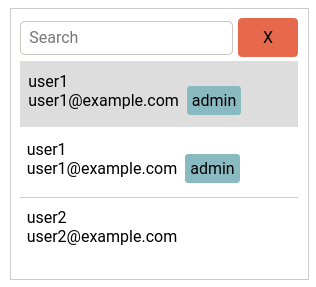
\includegraphics[width=70mm]{../img/picker_component.png}
  \caption{Vyrenderovaná komponenta jednoho vybírátka.}
  \label{fig:picker_component}
\end{figure}

\newpage
\subsection{Grafy}

Grafy jsou potřeba na stránce se statistiky. K tomu byla použita knihovna \textit{react-google-charts},
což, jak název napovídá, je port knihovny \textit{google-charts} do Reactu. Ta kromě obvyklích grafů umí
například i takzvaný kalendářový graf, jenž lze vidět na obrázku \ref{fig:google_charts}.

\begin{figure}[!htb] \centering
  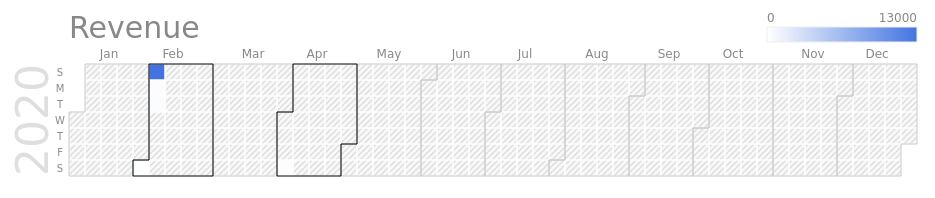
\includegraphics[width=145mm]{../img/google_charts.png}
  \caption{Kalendářový graf z knihovny react-google-charts.}
  \label{fig:google_charts}
\end{figure}


\chapter{Rozpoznávání SPZ}

\noindent
Jak již bylo řečeno v kapitole \ref{archtech}, mobilní aplikace pořídí snímek,
pošle ho backendu, jenž ho pošle serveru s knihovnou OpenALPR, která
rozpozná SPZ a výsledek pošle zpět na backend. V této kapitole si popíšeme
mobilní aplikaci a server s OpenALPR.

\section{Zvyšování přesnosti} \label{reco_params}

\noindent
Přesnost je hodně ovlivněna osvětlením, proto při nasazení v prostředí s neideálním
osvětlením je dobré použít dodatečné světlo osvětlující SPZ.

\subsection{Cachování výsledků}

\noindent
Výsledek z knihovny OpenALPR je seznam dvojic udávající SPZ a šanci, že konkrétní SPZ je správně --
jak si OpenALPR věří ve výsledek. Je tudíž logické měření udělat víc a provést aritmetický průměr a
zvolit nejlepší výsledek.

K ukládání takto dočasných dat (přibližně počet měření krát 1 sekunda) se databáze nehodí, a proto
bylo zavedeno ukládání do mezipaměti. V současné chvíli se využívá prostá paměť backendu,
kde klíčem je $id$ zařízení. Díky tomu, že Node.js běží na jednom vlákně, nemusíme se bát souběhu
(angl. race-condition). Externí mezipaměť by bylo vhodné využít (např. Redis), pokud by se spouštělo více
instancí backendu a prováděl by se takzvaný \textit{load-balancing}.

Výchozí počet měření je 2, a lze ho upravit v konfiguraci backendu.

\subsection{Filtrování podle geometrického obsahu}

\noindent
Pokud OpenALPR nalezne SPZ, udá i její pozici ve zdrojovém obrázku.
Aby se tedy předešlo naskenování SPZ, které jsou například daleko, lze odfiltrovat SPZ
podle jejich obsahu v pixelech čtverečních. Konkrétní hodnota je potřeba odladit na místě skenování a
lze změnit ve webové aplikaci pro kterékoliv zařízení.


\section{Autentizace}

\noindent
Zařízení se autentifikuje naskenováním QR kódu, jenž lze najít ve webové aplikaci. Ten obsahuje
JSON řetězec s aktivačním heslem, pomocí kterého se zařízení přihlásí do systému a získa svou konfiguraci.

Samotné skenování QR kódu je provedeno externí aplikací Barcode Scanner od vývojáře
Zxing Team, která lze nainstalovat z Play Store.

Konkrétní mechnismus komunikace s touto externí byl převzán. \citep[][]{QrScan}

\section{Volba zařízení pro mobilní aplikaci}

\noindent
Co se týče hardwarového vybavení snímacího zařízení, tak je vyžadována přední kamera
s rozlišením alespoň 1000 na 1000 pixelů. Bližší informace ohledně a zdůvodnění zmenšení jsou v sekci \ref{app_resizing}.
Procesor, RAM i vnitřní paměť může být libovolná -- kterékoliv
dnešní nové zařízení bohatě postačí (za předpokladu, že vnitřní paměť není zaplněná).
Minimální verze Androidu je 5 (SDK 21).

Autorovi se nepodařilo najít způsob, jak zároveň pořizovat v pravidelném intervalu snímky
a mít zařízení uzamknuté proti přístupu. K zajištění pořizování snímků si hlavní
obrazovka aplikace řekně systému Android o zabránění uzamknutí.

To má dva následky. První je, že zařízení by nemělo mít OLED displej, aby nedošlo k takzvanému
\textit{burn-in}. \citep[][]{OledBurnIn} Druhý je, že zařízení by mělo být v produkčním provozu
bezpečně uzavřeno v krabičce, nebo by se mělo nacházet na bezpečném místě, aby se předešlo
nepovolené manipulaci.

\section{Životní cyklus mobilní aplikace}

\noindent
Na obrázku \ref{fig:app_lifecycle} lze vidět životní cyklus mobilní aplikace.
Proces neprobíhá na jednom vlákně. Jakmile se pořídí fotografie, tak začně odpočet kolem jedné
sekundy, po kterém se pořídí další, a zároveň se už posílá první fotografie.
Změní-li se konfigurace na backendu, tak je poslána zařízení při dalším kontaktu, jinak
konfigurace poslána není.

\begin{figure}[!htb] \centering
  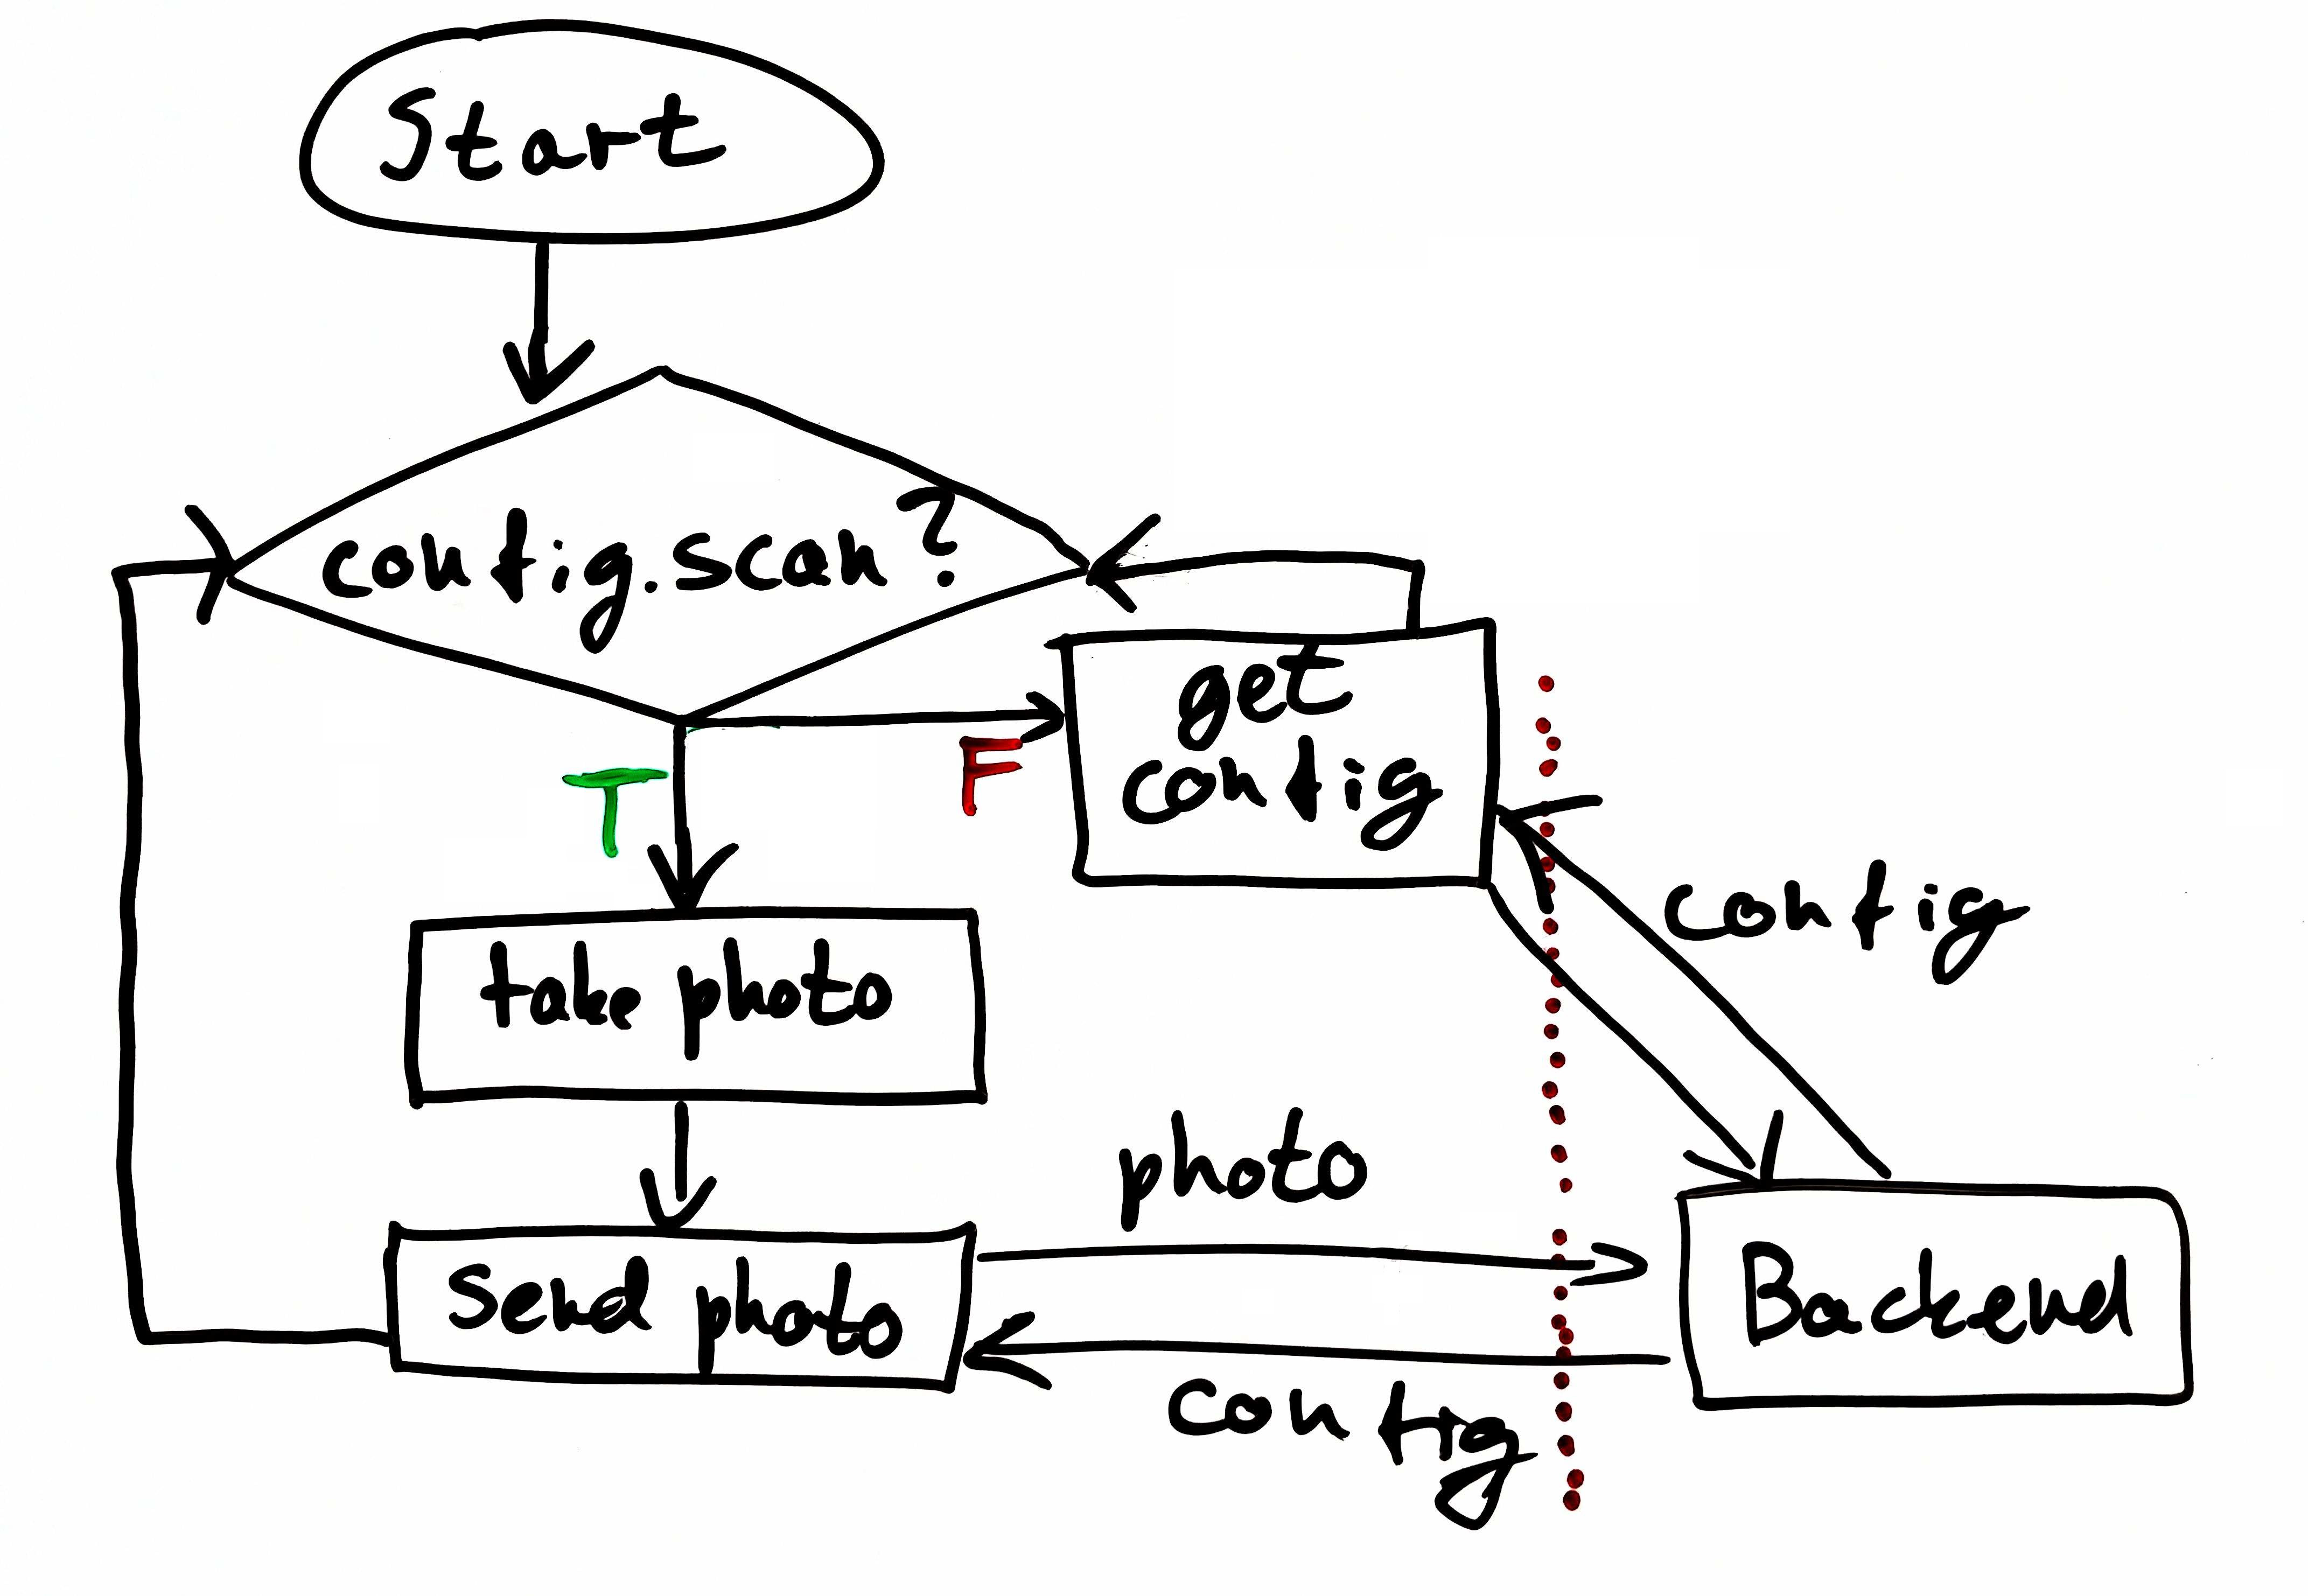
\includegraphics[width=135mm]{../img/app_lifecycle.jpg}
  \caption{Životní cycklus mobilní aplikace.}
  \label{fig:app_lifecycle}
\end{figure}

\section{Optimalizace velikosti přenesených dat} \label{app_resizing}

\noindent
Aby se ušetřilo na přenesených datech a aby rozpoznání proběhlo rychleji,
mobilní aplikace zmenší snímek
na nastavitelnou hodnotu
Tuto funkci poskytuje metoda \textit{createScaledBitmap} v třídě \textit{android.graphics.Bitmap}.

V závislosti na poměru stran snímků největšího rozlišení fotoaparátu,
může být potřeba hodnotu zmenšení změnit.
Základní hodnota je 1300x1000 pixelů, protože aplikace byla testována na
zařízení s fotoaparátem o roslišení 4356x3492 pixelů (poměr stran je 4:3).

Ušetření je opravdu veliké. Při testu s fotoaparátem o rozlišení 4356x3492 pixelů
byla průměrná velikost nezmenšených snímků $1,9$MB (JPG, $N=50$, $\sigma=0,325$).
Průměrná velikost snímků zmenšených na 1300x1000 pixelů byla
$0,15$MB (JPG, $N=50$, $\sigma=0,024$). Kdyby byla frekvence snímání jeden snímek za sekundu,
tak by bez optimalizací byl objem přenesených dat za jeden den $164,16$GB ($3600\cdot24\cdot1,9$MB).
Při stejné frekvenci s optimalizacemi by byl objem přenesených dat za jeden den
$12,96$GB ($3600\cdot24\cdot0,15$MB), což je $7,9$\% objemu bez optimalizací.

\section{Uživatelské rozhraní mobilní aplikace}

\noindent
Uživatelské rozhraní se skládá ze dvou obrazovek. Na obrázcích \ref{fig:app_ui}
lze vidět obě -- hlavní obrazovku a nastavení.

\begin{figure}[!htb] \centering
  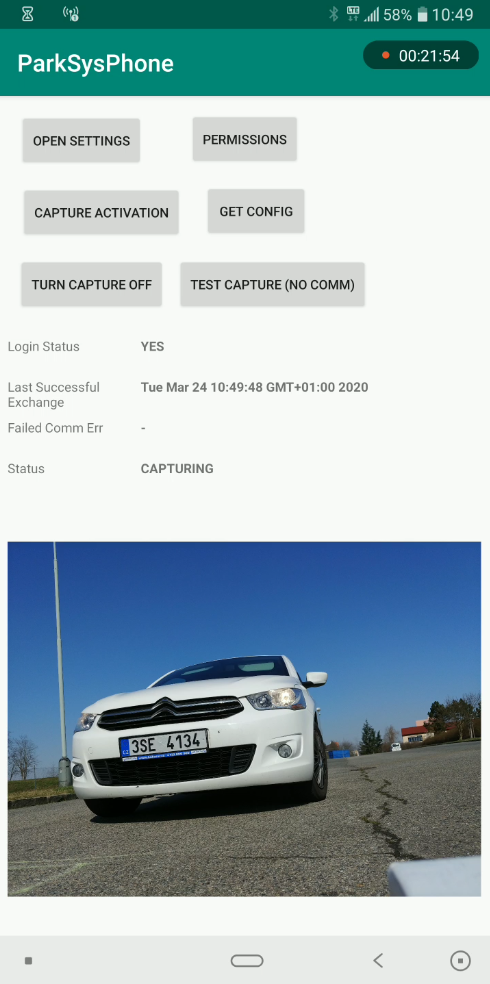
\includegraphics[width=70mm]{../img/app_mainscreen.png}
  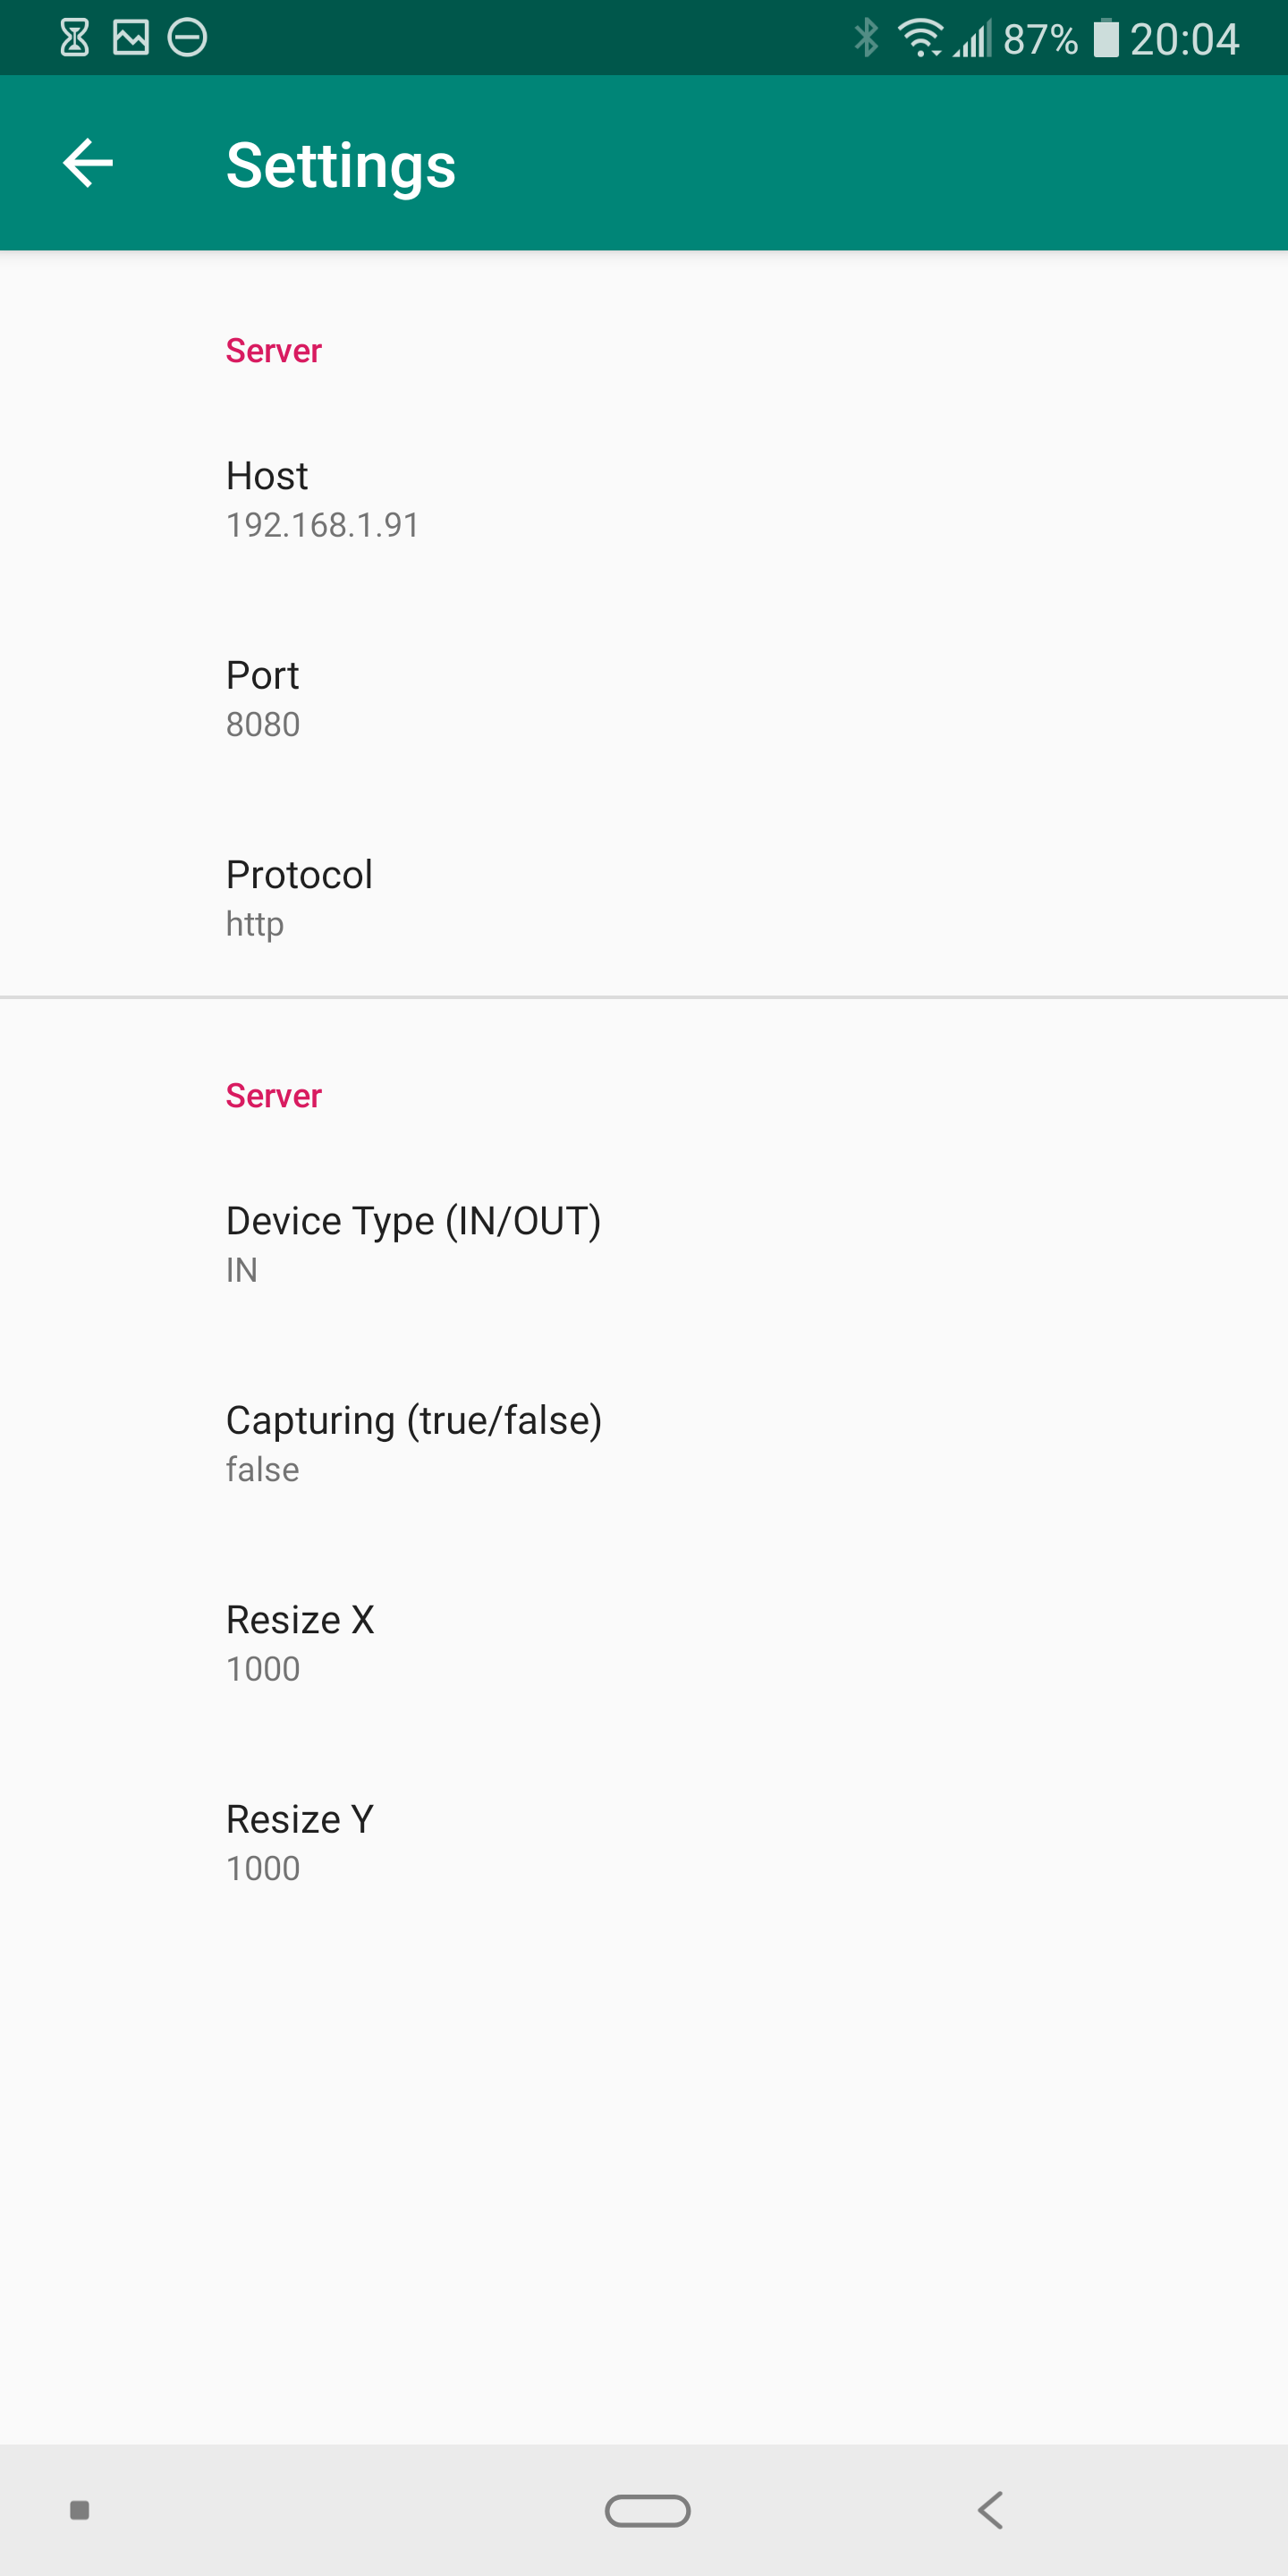
\includegraphics[width=70mm]{../img/app_settings.png}
  \caption[Rozhraní mobilní aplikace.]{
    Rozhraní mobilní aplikace.
    Hlavní obrazovka zobrazuje poslední snímek a status komunikace s backendem.
    V nastavení lze nastavit adresu backendu a vybrat si mezi HTTP a HTTPS a
    zobrazit nastavení typu zařízení a úpravy snímku.}
  \label{fig:app_ui}
\end{figure}


\section{Implementační detaily mobilní aplikace}

\subsection{Komunikace s backendem}

\noindent
Ke komunikaci přes HTTP využívá aplikace knihovnu Volley, která je doporučena
v Android dokumentaci. Princip použití je takový, že si vytvoříme
\textit{singleton} obstarávající frontu žádostí, kterému předáváme HTTP žádosti s
\textit{callback} funkcí obsluhující odpověď. \citep[][]{Volley1}

\subsection{Ukládání snímků}

\noindent
Snímky se ukládají do paměti určené pro aplikaci. Kdyby se použily dočasné soubory,
mohlo by se stát, že je systém před posláním nemilosrdně smaže.
\citep[][]{AndroidMem}
Aplikace tedy musí obstarávat i mazání souborů, což se provádí
ihned po odeslání snímku na backend.

% 
\chapter{Uživalteská dokumentace} \label{uzivatelska_dokumentace}


\chapter{Instalace} \label{analyza}

Instalace celého systému je velice jednoduchá. Pro distribuci je použit nástroj
Docker \citep[viz][]{DockerDocs}, který zajistí kompilaci, spuštění, propojení všech částí a odhalení
potřebných služeb ven na internet.

Kromě Backendu, Frontendu, OpenALPR Server a MongoDB používá tato distribuce
Dockerem populární HTTP server NGINX pro SSL a reverse proxy. Vnitřní HTTP komunikace
tak nemusí být zabezpečena.

\subsubsection*{Postup Instalace}

\begin{enumerate}
  \item Po stažení git repozitáře se zdrojovým kódem nastavíme submoduly:\\
  \begin{lstlisting}
    $ git submodule init
    $ git submodule update --remote --recursive
  \end{lstlisting}
  \item Dle potřeby upravíme soubor \textit{/docker-compose.yml} kvůli hostname, SSL certifikátům pro NGINX apod.
  \item Celý systém spustíme.\\
  \begin{lstlisting}
    $ docker-compose up
  \end{lstlisting}
\end{enumerate}

Poslední krok může trvat i několik minut v závislosti na rychlosti internetového
přípojení. Protože Docker zabalí vše včetně systémových závislostí, velikost
výsledných imagů je $1,4$GB.


\chapter*{Závěr}
\addcontentsline{toc}{chapter}{Závěr}

Výsledný projekt splňuje celé zádání kromě jednoho bodu -- konkrétně se jedná o
různý provoz
o svátích a podobných dnech (viz \ref{missing1}). Implementace takovéto funkcionality
vyžaduje implementovat kalendář.
Co se týče rozpoznávání SPZ, statistik, samotných pravidel a filtrů vozidel,
tak zde je vše implementováno a funguje skvěle.
Při prohlížení záznamů parkování lze nahlédnout na výřez SPZ z pořízeného snímku.
Navíc lze pravidla a filtry simulovat pro libovolné vozidlo.

Vývoj byl díky vhodně zvoleným technologiím poměrně rychlý a bezbolestný.
V jeho průběhu nedošlo k žádnému backtrackování kvůli předchozím rozhodnutím.
Projekt je bez velkých obtíží rozšiřitelný a pozměnitelný.
Dalším rozšířením, aby projekt byl plnohodnotný parkovací systém, by byla
integrace s platebním terminálem a závorou.


%%% Seznam použité literatury
%%% Seznam použité literatury (bibliografie)
%%%
%%% Pro vytváření bibliografie používáme bibTeX. Ten zpracovává
%%% citace v textu (např. makro \cite{...}) a vyhledává k nim literaturu
%%% v souboru literatura.bib.
%%%
%%% Příkaz \bibliographystyle určuje, jakým stylem budou citovány odkazy
%%% v textu. V závorce je název zvoleného souboru .bst. Styly plainnat
%%% a unsrt jsou standardní součástí latexových distribucí. Styl czplainnat
%%% je dodáván s touto šablonou a bibTeX ho hledá v aktuálním adresáři.

\bibliographystyle{czplainnat}    %% Autor (rok) s českými spojkami
% \bibliographystyle{plainnat}    %% Autor (rok) s anglickými spojkami
% \bibliographystyle{unsrt}       %% [číslo]

\renewcommand{\bibname}{Seznam použité literatury}

%%% Vytvoření seznamu literatury. Pozor, pokud jste necitovali ani jednu
%%% položku, seznam se automaticky vynechá.

\bibliography{literatura}

%%% Kdybyste chtěli bibliografii vytvářet ručně (bez bibTeXu), lze to udělat
%%% následovně. V takovém případě se řiďte normou ISO 690 a zvyklostmi v oboru.

% \begin{thebibliography}{99}
%
% \bibitem{lamport94}
%   {\sc Lamport,} Leslie.
%   \emph{\LaTeX: A Document Preparation System}.
%   2. vydání.
%   Massachusetts: Addison Wesley, 1994.
%   ISBN 0-201-52983-1.
%
% \end{thebibliography}


%%% Obrázky v bakalářské práci
%%% (pokud jich je malé množství, obvykle není třeba seznam uvádět)
\listoffigures

%%% Tabulky v bakalářské práci (opět nemusí být nutné uvádět)
%%% U matematických prací může být lepší přemístit seznam tabulek na začátek práce.
%\listoftables

%%% Použité zkratky v bakalářské práci (opět nemusí být nutné uvádět)
%%% U matematických prací může být lepší přemístit seznam zkratek na začátek práce.
% \chapwithtoc{Seznam použitých zkratek}

%%% Přílohy k bakalářské práci, existují-li. Každá příloha musí být alespoň jednou
%%% odkazována z vlastního textu práce. Přílohy se číslují.
%%%
%%% Do tištěné verze se spíše hodí přílohy, které lze číst a prohlížet (dodatečné
%%% tabulky a grafy, různé textové doplňky, ukázky výstupů z počítačových programů,
%%% apod.). Do elektronické verze se hodí přílohy, které budou spíše používány
%%% v elektronické podobě než čteny (zdrojové kódy programů, datové soubory,
%%% interaktivní grafy apod.). Elektronické přílohy se nahrávají do SISu a lze
%%% je také do práce vložit na CD/DVD. Povolené formáty souborů specifikuje
%%% opatření rektora č. 72/2017.
% \appendix
% \chapter{Přílohy}
% \include{prilohy/prilohy.tex}

\appendix
\newpage
\pdfpagewidth=33.1in
\pdfpageheight=14in
\setlength\textwidth{33.1in}
\setlength\linewidth{33.1in}

\chapter{GraphQL Schema} \label{app:a:graphql_schema}
\noindent

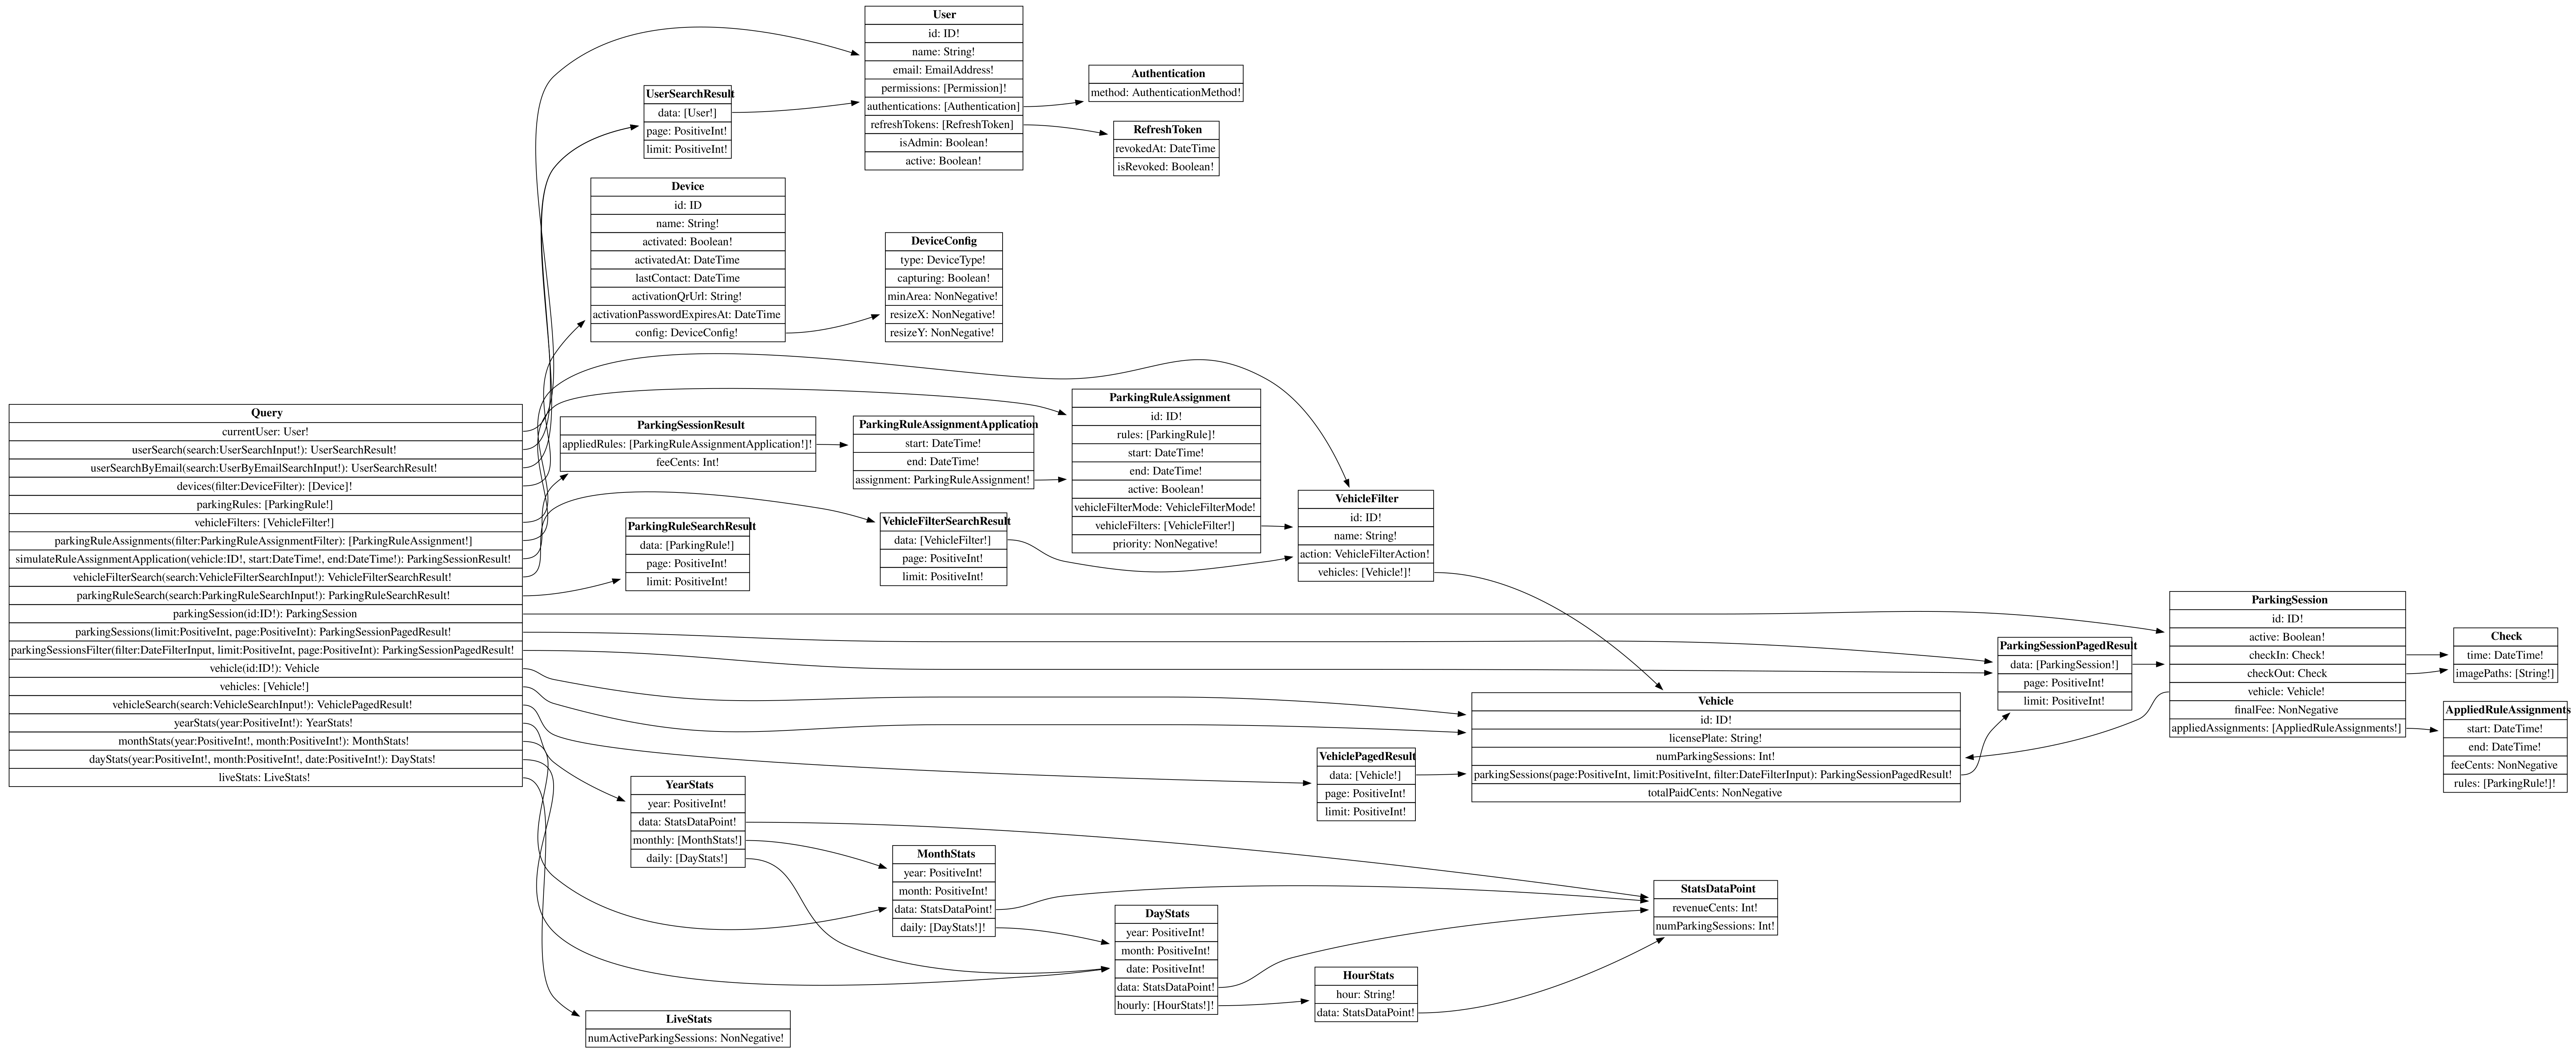
\includegraphics[width=30in]{../img/gql_query_schema.png}
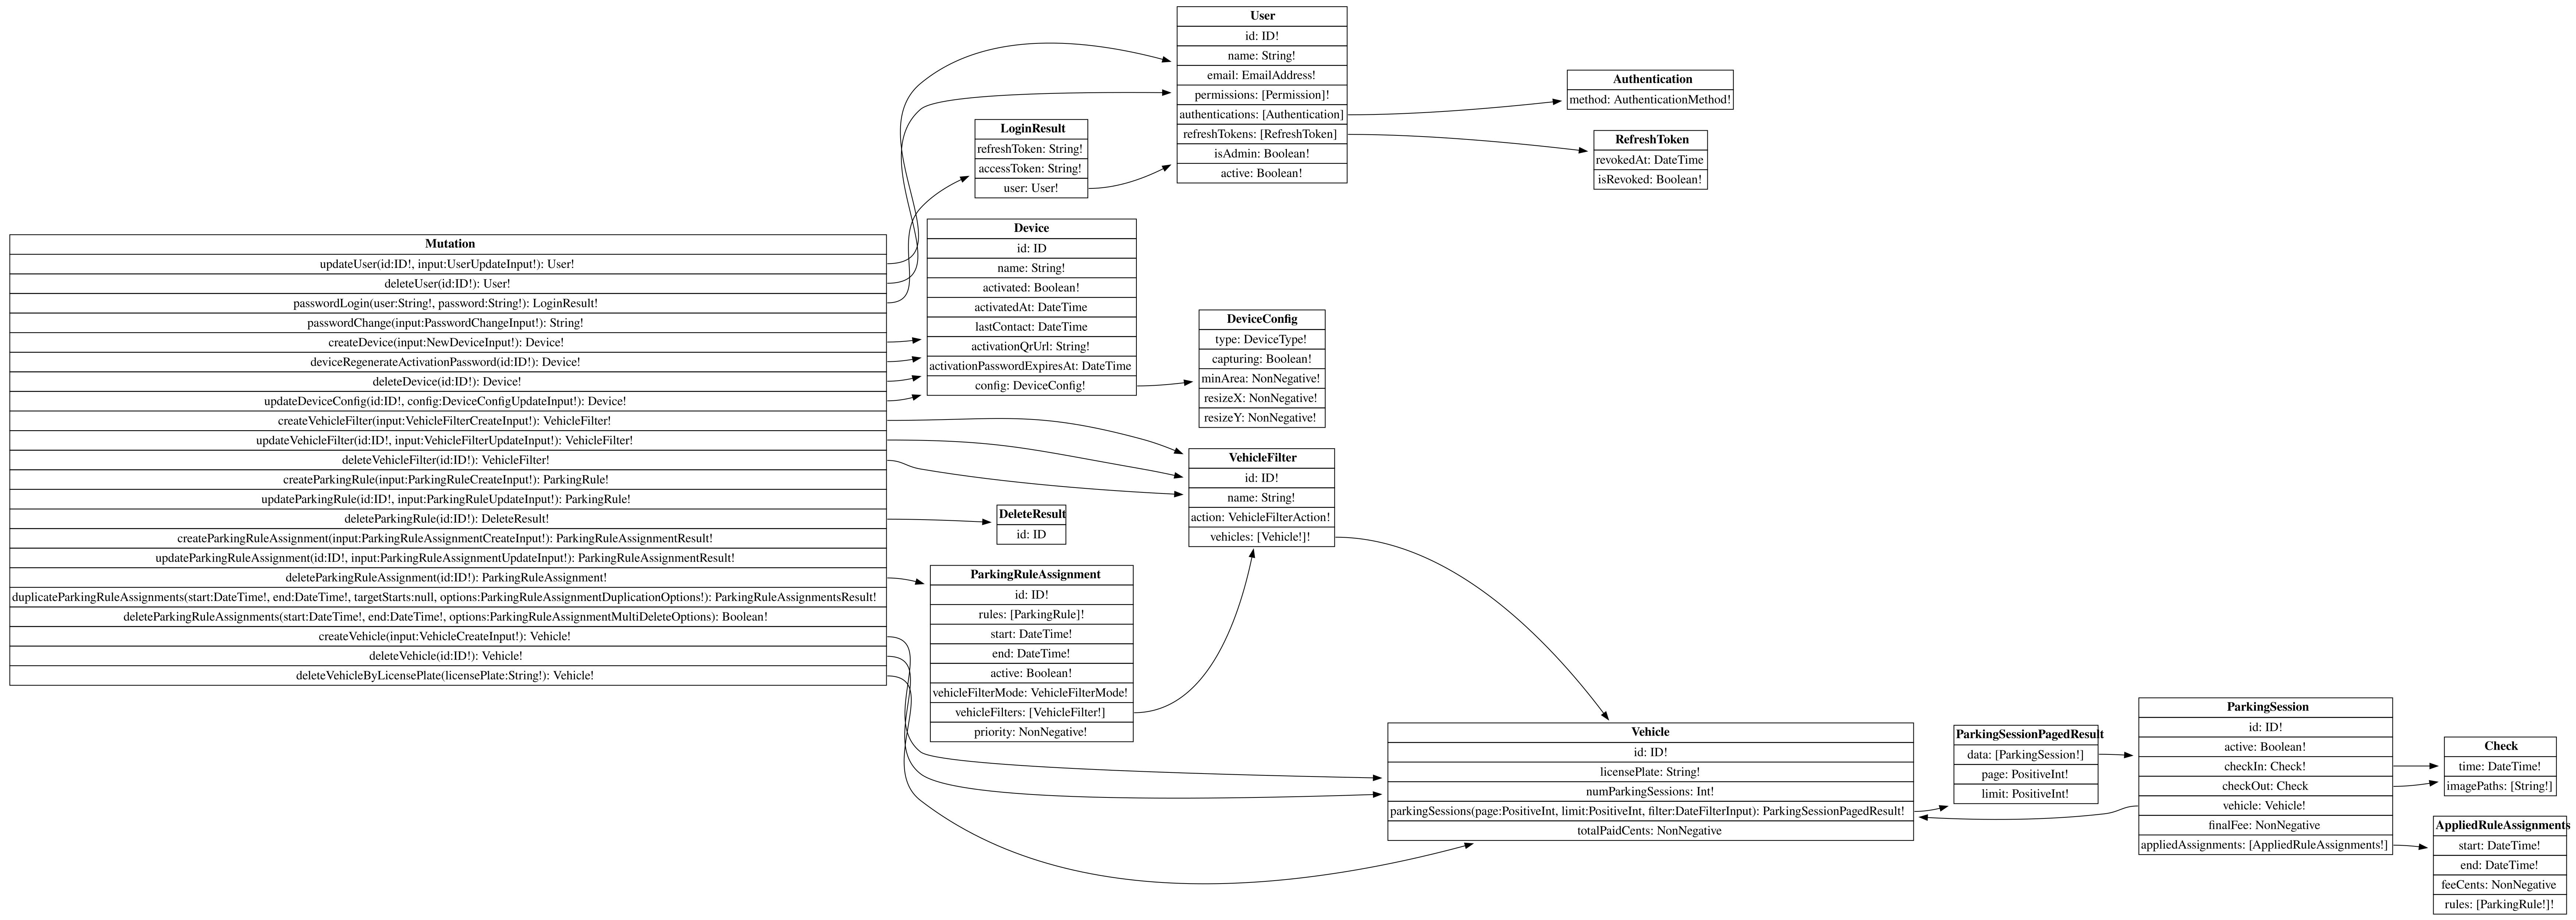
\includegraphics[width=30in]{../img/gql_mutation_schema.png}

% \openright
\end{document}
